% ===================== main.tex =====================
\documentclass[11pt,a4paper]{article}
\usepackage[utf8]{inputenc}
\usepackage[T1]{fontenc}
\usepackage{mathptmx}
\usepackage[margin=2.5cm]{geometry}
\usepackage{microtype}
\usepackage{amsmath,amssymb}
\usepackage{booktabs,array,multirow}
\usepackage{graphicx}
\usepackage{xcolor}
\usepackage[numbers,sort&compress]{natbib}
\usepackage{caption}
\usepackage[hidelinks]{hyperref}

% NOTE: replace the class, margins and bibliography style with the journal template once the journal is chosen.

% ---- numbers: a generated numbers.tex overrides these defaults ----
\IfFileExists{numbers.tex}{\input{numbers.tex}}{}
\providecommand{\Nimages}{3{,}500}
\providecommand{\Nmodels}{12}
\providecommand{\Nstrata}{13}
\providecommand{\Ncalls}{11{,}750}
\providecommand{\Nresponses}{141{,}000}

% ---- draft tags: set \showtagsfalse for the final version ----
\newif\ifshowtags
\showtagstrue
% \rad marks text that depends on the radiology arm (blue in the draft, plain in the final version)
\newcommand{\rad}[1]{\ifshowtags{\color{blue}#1}\else#1\fi}
% \PH marks a number or word to be bound to the result files (red in the draft, plain in the final version)
\newcommand{\PH}[1]{\ifshowtags{\color{red}#1}\else#1\fi}
% \TODO marks a missing passage (shown in the draft, removed in the final version)
\newcommand{\TODO}[1]{\ifshowtags{\color{red}[#1]}\else\fi}

% ---- metric names (usable in text and in mathematics) ----
\newcommand{\SMHR}{\ensuremath{\mathrm{SMHR}}}
\newcommand{\CHR}{\ensuremath{\mathrm{CHR}}}
\newcommand{\SRI}{\ensuremath{\mathrm{SRI}}}

\title{MedViHall: A Cross-Modality Benchmark for Severity-Weighted Hallucination Evaluation in Medical Vision-Language Models}
% NOTE: provisional title. Author list and affiliations to be supplied; co-authors are not assumed.
\author{Anuruddha Paul\\ \small KIIT Deemed to be University, Bhubaneswar, India}
\date{}

\begin{document}
\maketitle

\begin{abstract}
\TODO{Abstract to be written last, from audited results.}
\end{abstract}

\section{Introduction}
\label{sec:intro}

% NOTE: numbers inside \PH{...} come from claim_audit_report.md (recomputed from raw judge files) and must be bound to numbers.tex.
% NOTE: radiology: 1,073 of 1,200 radiology identifiers point to one image file (claim_audit_report.md, X1). Every radiology-dependent statement carries \rad{}.
% NOTE: the Introduction states 3,500 images through \Nimages; reconsider this figure once the radiology decision is made (2,405 distinct image files at present).

Vision-language models (VLMs) are now proposed as assistants for the interpretation of medical images. A single model can accept an image together with a natural-language instruction and return a free-text description, an answer to a targeted question, or a suggested diagnosis and next step. Two families of models are in use. General-purpose VLMs are trained on broad image--text corpora and are applied to medical images without specific adaptation. Domain-adapted models, for example LLaVA-Med \citep{li2023llavamed}, CheXagent \citep{chen2024chexagent} and HuatuoGPT-Vision \citep{chen2024huatuogptvision}, start from a general architecture and are further trained on biomedical image--text data. The two families differ in training data, in the extent of adaptation and in the clinical areas they target, and it is not established in advance which of them produces the more reliable output for a given imaging domain.

A recurrent failure of both families is hallucination, that is, generated content that is not supported by the input image or that contradicts it \citep{ji2023survey,bai2024hallucination}. In general-domain settings, a hallucination is usually counted as an error of uniform weight. In clinical imaging this convention is inadequate, because the consequence of an error depends on its type. A lesion reported on an image that contains none can lead to unnecessary investigation or treatment. A finding that is present in the image but absent from the report can delay care. An incorrect anatomical location, a misjudged severity, or a plausible but unsupported diagnostic inference each carry a different clinical risk, and a non-committal answer that identifies nothing carries a different risk again. A benchmark that reports a single error rate treats these cases as interchangeable and therefore cannot indicate how harmful the errors of a model are, only how frequent they are.

Prior work has addressed parts of this problem. Med-HallMark and its MediHall Score assign hallucinations to five levels of severity and score model output accordingly, for medical visual question answering and report generation \citep{chen2024medhallmark}. CREST, a risk-weighted score defined over a taxonomy of twelve error types that physicians graded as low, medium or high clinical risk, was developed for chest radiograph report impressions \citep{crest2025medrxiv}. HalluCXR evaluates six models on 856 frontal chest radiographs with an eight-category taxonomy and three severity levels, and reports that normal radiographs drew the most severe hallucinations \citep{wang2026hallucxr}. ClinHallu decomposes the reasoning of a medical model into stages in order to locate where hallucinations arise \citep{yang2026clinhallu}. MedHEval groups hallucinations by cause and evaluates seven mitigation methods on radiological data \citep{chang2025medheval}. CARES assesses several dimensions of trustworthiness, hallucination among them, over a large collection of question--answer pairs spanning many imaging modalities \citep{xia2024cares}. Related studies examine whether models abandon a correct image-based answer under social pressure, and report both that medical fine-tuning can increase this vulnerability \citep{xu2025sycophancy} and that the models which hallucinate least can be the most prone to yield to such pressure \citep{aranya2026grounding}. Severity-aware scoring and taxonomies of hallucination therefore have precedent, and neither is presented here as new in itself.

Three limitations of the existing evidence motivate the present work. First, the benchmarks that grade hallucinations by clinical consequence are concentrated in radiology, and in chest radiography in particular. Dermatology, histopathology and ophthalmology are evaluated in several studies, but these differ in task and in the treatment of error, so that results obtained in one domain cannot be placed beside results obtained in another. Second, a severity-weighted score is usually reported as an absolute number. Such a number has no stable interpretation across modalities, because the base rate of abnormal findings, the typical length of a response and the difficulty of the images all differ, and a value that is low for one modality may be high for another. A comparison of domain-adapted models with general-purpose models in each modality requires a common reference. Third, the evidence on whether domain adaptation reduces or increases hallucination is mixed. The studies cited above point in different directions depending on the task, the models and the pressure applied, and the question is seldom examined with confidence intervals that treat the image, and not the response, as the unit of independent evidence.

This article introduces MedViHall, a cross-modality benchmark for severity-weighted hallucination evaluation of medical VLMs, and uses it to examine these three points. The benchmark contains \Nimages{} images drawn from public datasets in four imaging modalities: chest radiography, dermatology, histopathology and ophthalmology. The images are organised into \Nstrata{} design strata that separate normal images from images with abnormal findings of defined types, so that the evaluation can distinguish a model that invents findings from one that misses them. Each image is presented to each model through up to four query types. The first requests an open-ended report. The second asks a targeted yes/no question. The third asks for a diagnosis and the immediate action it would imply. The fourth, applied to normal images only, states a false premise that asserts an abnormality and asks the model to proceed from it. This protocol elicits the behaviours that matter in practice, namely spontaneous description, answering under a direct question, committing to a diagnosis, and resisting an incorrect clinical premise. Twelve open-weight VLMs, nine general-purpose and three domain-adapted, were evaluated, which yielded \Nresponses{} responses.

Each response is decomposed into atomic claims, and each claim is assigned to one of seven hallucination classes: fabrication, omission, misclassification, severity distortion, anatomical confusion, evasion and clinical reasoning error. Five of these classes correspond to categories already used for chest radiography \citep{wang2026hallucxr}; misclassification and evasion are not among the categories of that scheme. Each class carries a weight that reflects its assumed clinical consequence. The weights were assigned by the authors and are examined by sensitivity analysis rather than presented as clinically elicited values. Three metrics are derived from the labelled claims. The severity-weighted medical hallucination rate (\SMHR) is the mean weight over all claims, so that it increases with the frequency and with the severity of errors. The clinical hallucination rate (\CHR) is the proportion of responses that contain at least one fabrication or omission. The specialisation ratio index (\SRI) divides the \SMHR{} of a model in a given modality by that of the best general-purpose model in the same modality, so that a value above one indicates that the model hallucinates more, in the severity-weighted sense, than the strongest general-purpose reference. All intervals are obtained by resampling images.

The benchmark was used to answer four questions. Does the ranking of the models by \SMHR{} separate the models, once sampling uncertainty over images is taken into account? Do the domain-adapted models hallucinate less than the best general-purpose model in their respective modalities? How consistent are the rankings across modalities? Do inference-time mitigation strategies reduce \SMHR{} when each is compared with an appropriate baseline? The principal findings are as follows.
% NOTE: refresh every figure in the following paragraphs from the audited result files before submission.
The five general-purpose models with the lowest \SMHR{} obtain values between \PH{0.529} and \PH{0.562}. The first three of them are not separated from one another, so that no ordering within this group is supported; the remaining general-purpose models have a higher \SMHR{}. Each of the three domain-adapted models has a higher \SMHR{} than the best general-purpose model in each of the four modalities, with \SRI{} values from \PH{1.31} to \PH{1.85}, and all twelve intervals exclude one \rad{(three of the twelve cells are radiology cells, which depend on the unresolved image issue)}. The \SRI{} of every cell remains above one under equal class weights and under random perturbation of the class weights by up to \PH{30\%}. It is a comparison with the best of nine general-purpose models. It does not isolate the effect of medical adaptation, because the models differ in size, architecture and training data, and one of the three domain-adapted models scores better than at least one general-purpose model in every modality. The values for LLaVA-Med are an upper bound, because about \PH{one third} of its responses begin in mid-sentence as a consequence of a decoding defect.
% NOTE: confirm the LLaVA-Med repair status (rerun or report both numbers) before this sentence is final.
Rankings by \SMHR{} in dermatology, histopathology and ophthalmology are positively correlated across the twelve models (Spearman correlations from \PH{0.66} to \PH{0.81}), but the correlations are weaker among the nine general-purpose models alone, and they therefore reflect in part the separation between the two families; the transfer of rankings to and from radiology could not be assessed \rad{}. The \CHR{} does not order the models as \SMHR{} does, which supports the reporting of both. Contrastive decoding lowered the \SMHR{} of one domain-adapted model, HuatuoGPT-Vision, against both the benchmark baseline and a matched greedy baseline, with and without the radiology images, and it was the only mitigation effect with this property. Retrieval-augmented prompting did not lower \SMHR{} consistently, and it increased the share of responses containing a fabrication or omission for four of the five models examined.

The contributions of this article are the following.
\begin{enumerate}
  \item A seven-class taxonomy of hallucination in medical image interpretation with explicit class weights, adapted from categories in use for chest radiography and extended to the other modalities, and three metrics, \SMHR, \CHR{} and \SRI, that report error frequency, error severity and the position of a model relative to a fixed general-purpose reference in each modality.
  \item A benchmark of \Nimages{} images in four modalities and \Nstrata{} design strata, with a query protocol that includes a false-premise query on normal images, and a two-layer pipeline that extracts claims and assigns them to the taxonomy.
  \item A measurement of the gap between domain-adapted and general-purpose models in each modality, accompanied by image-level bootstrap intervals, tests of which orderings the data support, a sensitivity analysis over the class weights, and an assessment of how far rankings agree across modalities.
  \item A comparison of two inference-time mitigation strategies, retrieval-augmented prompting and contrastive decoding, on five models, in which each strategy is compared with the benchmark baseline and with a matched greedy baseline, so that the effect of the strategy can be separated from the effect of the decoding setting.
  \item An audit of the automated labelling pipeline against annotations produced by six simulated annotators, which supports the detection of the presence of any hallucination at the level of the item and shows that the class-specific labels are not validated. No clinician annotation is included.
  % NOTE: item 5 must be revised if clinician annotation becomes available (Version A); the current wording follows annotation_report.md and annotation_paper_paragraphs.tex (Version B).
\end{enumerate}

The remainder of the article is organised as follows. Section~\ref{sec:related} reviews prior work on hallucination in general and in medical VLMs and on severity-aware evaluation. Section~\ref{sec:benchmark} describes the imaging data, the query protocol, the taxonomy and the metrics. Section~\ref{sec:setup} describes the models, the inference settings and the statistical procedures. Section~\ref{sec:results} reports the results, including the comparison between domain-adapted and general-purpose models, the behaviour of each modality, the stability of rankings and the mitigation experiments. Section~\ref{sec:validation} reports the audit of the labelling pipeline. Section~\ref{sec:discussion} discusses the findings, and Section~\ref{sec:limitations} states the limitations of the study, including the author-assigned class weights, the use of quantised models, the restriction to open-weight models, the dependence of the labels on a single local judge model and the incomplete validation of the class-specific labels.

\section{Related Work}
\label{sec:related}

% NOTE: packages required: booktabs. Sources are listed in refs_related.bib; items read only through related_work_report.md are marked in that file.

\subsection{Hallucination in vision-language models}
\label{subsec:rw_vlm}

Hallucination in image-conditioned text generation was first quantified for image captioning. The CHAIR metric measures how often a captioning model mentions objects that are absent from the image, and the accompanying analysis showed that the models with the best scores on standard sentence-level metrics do not always hallucinate least \citep{rohrbach2018chair}. For large vision-language models, POPE recasts the problem as a set of polling questions on the presence of objects. Its authors report that most of the models they tested frequently describe objects that do not correspond to the image, and that objects which occur often in instruction data or together with other objects in an image are particularly prone to being hallucinated \citep{li2023pope}. Surveys of hallucination in natural language generation and in multimodal language models document the causes, the evaluation methods and the mitigation approaches proposed so far \citep{ji2023survey,bai2024hallucination}. These benchmarks treat each error as a unit of equal weight and are built on natural images, in which the presence of an object can be verified from common knowledge. Neither condition holds in medical imaging, where the verification of a statement requires a ground truth derived from expert interpretation and where the consequence of an error depends on its type.

\subsection{Claim-level and automated evaluation}
\label{subsec:rw_claims}

Evaluating a long free-text response requires a unit of analysis smaller than the response. FActScore decomposes the output of a language model into short, self-contained claims and reports the share of claims supported by a trusted reference, together with an automated estimator that closely approximates human judgements \citep{min2023factscore}. The claim is also the unit of analysis in the present work. The reference, however, is a structured image-level ground truth and not a text corpus, and the score has to account for statements that a response fails to make, which a precision-oriented measure does not capture.

Automated judgement by a language model is the usual means of scaling such evaluation. In a general-purpose setting, a strong proprietary judge was found to agree with controlled expert preferences and with crowdsourced human preferences at a rate above 80\%, which matches the agreement observed between human raters \citep{zheng2023judge}. That result concerns a large judge and general conversational preferences. It does not transfer automatically to a smaller locally hosted judge applied to medical claims, and the labelling pipeline used here (Section~\ref{sec:benchmark}) is therefore examined separately in Section~\ref{sec:validation}.

\subsection{Medical vision-language models}
\label{subsec:rw_medvlm}

Domain-adapted VLMs start from a general architecture and are further trained on biomedical image--text data. LLaVA-Med was trained to act as an assistant for biomedical images \citep{li2023llavamed}. CheXagent was developed as a foundation model for the interpretation of chest radiographs \citep{chen2024chexagent}. HuatuoGPT-Vision was built by injecting medical visual knowledge into a multimodal language model at scale \citep{chen2024huatuogptvision}. The three models differ in scope. CheXagent targets one modality, whereas the other two address medical images in general. This difference is relevant to the interpretation of the specialisation results in Section~\ref{sec:results}, because the performance of CheXagent on dermatology, histopathology and ophthalmology images measures in part the transfer of a chest radiograph model to other domains.

\subsection{Hallucination benchmarks for medical vision-language models}
\label{subsec:rw_bench}

Several benchmarks examine hallucination in medical VLMs, and they differ in task, in scope and in the way an error is graded. Table~\ref{tab:related} summarises their main properties.

\begin{table}[t]
\centering
\small
\caption{Properties of benchmarks for hallucination in medical vision-language models, as stated in the cited sources. A dash indicates that the property was not established from the sources consulted.}
\label{tab:related}
\begin{tabular}{@{}p{2.3cm}p{4.9cm}p{3.5cm}p{3.1cm}@{}}
\toprule
Work & Scope and task & Models evaluated & Severity or risk grading \\
\midrule
\citet{wu2024halluvqa} & PMC-VQA, PathVQA and VQA-RAD recast as multiple-choice questions (FAKE, NOTA, image swap) & LLaVA variants including LLaVA-Med; GPT-4-turbo-vision & --- \\
\citet{chen2024medhallmark} & Medical VQA and report generation & --- & Five levels (MediHall Score) \\
\citet{gu2024medvh} & Five tasks, including long-form response generation & --- & --- \\
\citet{yan2025medhalltune} & Over 100,000 images and over 1,000,000 instruction pairs & Medical and general-purpose VLMs & Risk level, one of four criteria \\
\citet{chang2025medheval} & Close-ended and open-ended medical VQA, radiology; three causes of hallucination & 11 VLMs; 7 mitigation methods & --- \\
\citet{wang2026hallucxr} & 856 frontal chest radiographs; three query types; eight-category taxonomy & 6 models & Three levels, reported as the share of outputs with a level-3 hallucination \\
\citet{yang2026clinhallu} & Stage-wise decomposition of reasoning & --- & --- \\
\citet{crest2025medrxiv} & 685 chest radiograph cases; report impressions & 3 VLMs & Three clinical risk levels \\
\citet{xia2024cares} & 41,000 question--answer pairs, 16 modalities; trustworthiness & --- & --- \\
This work & \Nimages{} images, 4 modalities, up to 4 query types & \Nmodels{} VLMs & Seven classes with weights \\
\bottomrule
\end{tabular}
\end{table}

Wu et al.\ adapted three public medical VQA datasets into multiple-choice questions under three scenarios: nonsensical questions, questions whose correct option is replaced by ``none of the above'', and questions paired with an unrelated image. They found that domain fine-tuning did not guarantee resistance to hallucination, since LLaVA-Med performed worse than the general model from which it was derived \citep{wu2024halluvqa}. MedVH comprises five tasks that cover the comprehension of text and visual input as well as long-form response generation, and reports that the medical models it evaluated often hallucinate more than general-purpose ones \citep{gu2024medvh}. MedHallTune provides over 100,000 images and over 1,000,000 instruction pairs, with and without hallucinated content, and evaluates models on clinical accuracy, relevance, level of detail and risk level. Its authors report that fine-tuning on the dataset reduced hallucination \citep{yan2025medhalltune}. MedHEval groups hallucinations by cause into visual misinterpretation, knowledge deficiency and context misalignment, and evaluates 11 models together with seven mitigation techniques on medical VQA data \citep{chang2025medheval}.

Work on radiology is more detailed. HalluCXR evaluates six models on 856 frontal chest radiographs from MIMIC-CXR, with CheXpert labels as ground truth. Its taxonomy has eight categories: fabrication, omission, spatial error, severity distortion, reasoning error, template overfitting, self-contradiction and detail fabrication. Each hallucination receives a severity of 1 to 3, and severity is reported as the share of outputs that contain at least one hallucination of level 3. No aggregate severity-weighted score is computed. The study reports that normal radiographs drew the most severe hallucinations \citep{wang2026hallucxr}. Five of the seven classes of the present taxonomy correspond to categories of HalluCXR, and the taxonomy should be read as an adaptation and extension of that scheme and not as an independent construction. ClinHallu decomposes the reasoning of a medical model into stages in order to locate the stage at which a hallucination arises \citep{yang2026clinhallu}. CARES assesses several dimensions of trustworthiness over 41,000 question--answer pairs from 16 modalities, and is therefore broad in modality but not specific to hallucination \citep{xia2024cares}. The finding of HalluCXR that normal images are the most hazardous is consistent with the design of the present benchmark, in which a false-premise query is applied to normal images in every modality.
% NOTE: the HalluCXR taxonomy and severity definitions were read from the full text (Table 3, Section 3.4) in this session.

\subsection{Evaluation outside radiology}
\label{subsec:rw_nonrad}

Studies of other imaging domains have mostly examined capability, grounding or confidence, and few score hallucination as a first-class outcome. CARES includes dermoscopy and fundus images within its trustworthiness suite \citep{xia2024cares}. A preprint on histopathology reports pathologist-graded errors, hallucinations and clinical impact for four general-purpose multimodal models \citep{lami2026histopathology}, and a second study reports that a general-purpose model produces confident descriptions when given blank histology images \citep{hasan2026seeing}. A study of vision-language models on chest radiography, brain MRI and dermatology shows that frontier models invent diagnoses when no image is supplied, and that the invented diagnosis depends on the demographic descriptors in the prompt \citep{vohra2026hearsay}. An audit of six large vision-language models for fundus images assesses dependence on text, logical consistency and the fidelity of chain-of-thought reasoning \citep{zhang2026fundus}. These studies establish that hallucination in non-radiological domains is real and measurable. They differ from one another in task, in grading and in the models examined, so that their results cannot be compared directly. A single protocol applied to several of these domains, with both domain-adapted and general-purpose models, is what the present benchmark provides.
% NOTE: lami2026histopathology was read through the medRxiv API abstract by an earlier session (lit_update.bib); the full text was not read. Cite the findings only at the level of the abstract.

\subsection{Severity-aware evaluation}
\label{subsec:rw_severity}

Two works grade errors by their clinical consequence, and they are the closest antecedents of the metrics proposed here. The MediHall Score assigns each statement to one of five levels, namely catastrophic, critical, attribute, prompt-induced and minor hallucination, with scores of 0.0, 0.2, 0.4, 0.6 and 0.8, and a score of 1.0 for a correct statement. Scores are averaged over the sentences of a report and over the answers of a set \citep{chen2024medhallmark}. The score is therefore normalised by all statements, correct ones included, and is sensitive to the frequency of errors. CREST defines twelve error types for chest radiograph report impressions, in four groups: incorrect affirmations or negations, mishandled uncertainty, omitted findings or negative evidence, and fabricated findings. Physicians assigned each type a high, medium or low clinical risk, which is mapped to weights of 3, 2 and 1 and normalised to the interval from 0 to 1. A companion measure reports the share of errors that are high risk \citep{crest2025medrxiv}.

The present work differs from these scores in three respects, and shares an important property with the first. Like the MediHall Score, \SMHR{} is normalised by all units and not by the errors alone; its difference lies in the unit, which is the atomic claim extracted from the response and not the sentence. Because both scores are weighted error rates over the same classified units, they are expected to order models similarly, and a direct comparison on the present data is reported in Section~\ref{sec:results}. First, the taxonomy is defined in terms of the relation between a claim and the image, includes omission as an explicit class, and is applied unchanged to four modalities. Second, \SRI{} expresses the \SMHR{} of a model relative to a fixed general-purpose reference in the same modality, which permits a comparison of specialist and general models across modalities with different base rates. Third, the class weights are assigned by the authors. This is a limitation relative to CREST, whose risk levels were assigned by physicians. A sensitivity analysis over the weights is reported in Section~\ref{sec:results}, and it can establish only the stability of the conclusions with respect to the weights, not their clinical validity.
% NOTE: Section results must contain the SMHR / MediHall / CREST comparison (claim_audit_report.md, C075-C078): SMHR and the MediHall Score ranked the 12 models identically by construction; SMHR and CREST rho = 0.64 (permutation p = 0.03).

\subsection{Domain adaptation and hallucination}
\label{subsec:rw_special}

Evidence on whether domain adaptation reduces hallucination is mixed. Wu et al.\ and Gu et al.\ report that medical models can be less robust than general models \citep{wu2024halluvqa,gu2024medvh}. EchoBench, which covers 20 modalities, reports that many medical-specific models exceed 95\% sycophancy \citep{yuan2025echobench}, and a benchmark of 5,000 items built from PathVQA, SLAKE and VQA-RAD found that medical fine-tuning tends to increase the tendency of a model to abandon a correct image-based answer under social pressure, with failure rates up to 75\% \citep{xu2025sycophancy}. A study of six models, three general-purpose and three medical, on three VQA datasets found that the models which hallucinated least were the most prone to yield to user pressure, and that none of the evaluated models of 7--8 billion parameters performed well on both grounding and pressure resistance \citep{aranya2026grounding}.

Paired designs, which compare a medical model with the general model from which it was derived, give a less uniform picture. A study of two such pairs, LLaVA-1.6 with LLaVA-Med and Gemma-3 with MedGemma, on four binary tasks in brain MRI, chest radiography, dermoscopy and histopathology found no reliable improvement from medical fine-tuning, with results that depended on the task and on the wording of the prompt \citep{mclaughlin2026knowledge}. A behavioural audit on brain MRI that included a base-versus-specialist pair found that medical adaptation improved the detection of tumours, while hallucination and abstention varied separately from accuracy \citep{sabbaghziarani2026confident}. These studies differ in task, in the way hallucination is measured and in the models included, and their results are not directly comparable with one another or with the present study. They indicate that a comparison of domain-adapted and general models should be reported as a measurement conditional on the models, the task and the metric, and that a design which does not contain base--specialist pairs cannot attribute a difference to the adaptation itself. The comparison in Section~\ref{sec:results} is formulated in this way: it compares each domain-adapted model with the best of nine general-purpose models and does not isolate the effect of medical adaptation.

\subsection{Calibration of stated confidence}
\label{subsec:rw_calibration}

Three of the four query types in the present protocol request a confidence value, which allows the calibration of the stated confidence to be examined alongside hallucination. Studies of medical VQA report that overconfidence persists across model families and is not removed by increasing scale or by prompting, that post-hoc calibration is more effective than prompt-based elicitation, and that signals from hallucination detection can improve calibration \citep{byun2026overconfidence}. A study of uncertainty methods over twelve VLMs and eight modalities reports that uncertainty is not a safety net for clinical VQA \citep{fazla2026uncertainty}, and a benchmark of calibration in medical VLMs examines classification across three modalities \citep{sharifdeen2026mvcbench}. The calibration experiments of the present study are reported in Section~\ref{subsec:res_calibration}. They vary the decoding setting, which, to our knowledge, was not varied in these studies.
% NOTE: Byun et al. was read at abstract level in this session. The statement about decoding settings follows claims_at_risk.md (section 5); re-run the literature search before submission.

\subsection{Mitigation of hallucination}
\label{subsec:rw_mitigation}

Mitigation strategies for VLMs act on the inputs, on the decoding procedure or on the model. Visual contrastive decoding is a training-free method that compares the output probabilities obtained from the original image with those obtained from a deliberately degraded version, and thereby steers generation towards content supported by the visual evidence \citep{leng2024vcd}. Retrieval-augmented generation supplies external text to the model at inference time \citep{lewis2020rag}. In the medical domain, MedHEval evaluates seven mitigation techniques that act on decoding or attention on 11 models, using radiological data \citep{chang2025medheval}, MedHallTune uses instruction tuning \citep{yan2025medhalltune}, and a single-call prompting method that removes social cues before the model answers has been proposed for sycophancy \citep{xu2025sycophancy}. A preprint on chest radiograph report generation reports that retrieval can itself induce hallucination when the retrieved context does not match the image \citep{idoko2026retrieval}. A mitigation experiment requires a baseline generated under the same decoding configuration as the mitigated arm, because a change in the decoding setting can alter the output independently of the strategy under test. The experiments in Section~\ref{sec:results} therefore report each strategy against two baselines, the benchmark response and a matched greedy response, and state the decoding configuration of every arm.

\subsection{Positioning of the present work}
\label{subsec:rw_position}

Severity-aware scoring, taxonomies of hallucination, benchmarks for medical hallucination, comparisons of domain-adapted with general models and studies of mitigation all have precedents, and none of them is presented here as new in itself. Localising the stage at which a hallucination arises is the subject of ClinHallu \citep{yang2026clinhallu} and is not attempted here. The contribution of the present work lies in the combination of a single taxonomy, a single query protocol and a single set of claim-level metrics applied to four imaging modalities for both domain-adapted and general-purpose models, in a reference-normalised index that supports comparison across modalities, in intervals that treat the image as the unit of independent evidence, and in a mitigation comparison in which each strategy is reported against two baselines. Among the works reviewed above, those that grade errors by clinical consequence were developed for report generation or for a single modality, and for several of the broader benchmarks the modality coverage and the grading scheme could not be established from the sources consulted (Table~\ref{tab:related}). A literature search should be repeated shortly before submission, since the number of relevant studies is increasing quickly.

% ===================== sec_benchmark.tex =====================
% NOTE (revision 2): rewritten against the pipeline scripts (stage1_extract_claims.py, stage2_*.py, stage3_layer2_judge.py, compute_model_metrics.py) and claim_audit_report.md. Changes from revision 1: G1020 added as a source; abnormal strata defined; reference-label fields listed as passed to the judge; Layer 1 now supplies omissions only and the judge classifies all claims of a response in one call; combination rule and omission handling stated; coverage figures corrected (histopathology 53.5 per cent, not 42); the judge's severity sub-score removed (the implemented prompt does not return one).
\section{Benchmark and Metric}\label{sec:benchmark}

\begin{figure}[t]
  \centering
  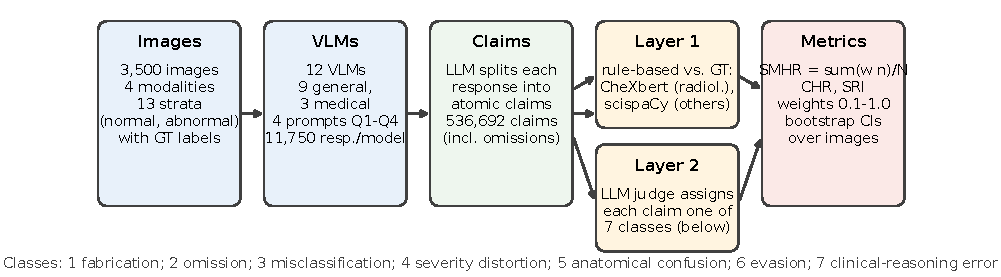
\includegraphics[width=\textwidth]{paper_figures/fig01_overview.pdf}
  \caption{Overview of the MedViHall evaluation. Images from four modalities are presented to twelve vision-language models. Each response is divided into atomic claims by a language model. An automated first layer compares the response with structured reference labels and reports omitted findings, and a second layer, a language-model judge, classifies each claim. Claim-level verdicts and omissions are weighted by class and aggregated into severity-weighted metrics.}
  \label{fig:overview}
\end{figure}

\subsection{Imaging data}\label{sec:data}
The benchmark covers four imaging modalities that differ in how the images are formed, in the clinical questions put to them, and in the structure of their reference labels: chest radiography, dermoscopy, histopathology and colour fundus photography. For each modality we used public datasets that provide reference labels. Chest radiographs are taken from CheXpert v1.0~\citep{irvin2019chexpert}. Dermoscopic images come from the ISIC 2020 dataset~\citep{rotemberg2021isic} and from HAM10000~\citep{tschandl2018ham10000}. Histopathology images are patches from PatchCamelyon~\citep{veeling2018pcam} and from NCT-CRC-HE-100K~\citep{kather2019nct}. Fundus images come from REFUGE~\citep{orlando2020refuge}, ORIGA-light~\citep{zhang2010origa} and G1020~\citep{bajwa2020g1020}.

The benchmark contains \Nimages{} image identifiers: 1{,}200 radiographs, 900 dermoscopic images, 800 histopathology patches and 600 fundus photographs. They were drawn by stratified sampling with a fixed seed (42) and are divided into \Nstrata{} design strata (Table~\ref{tab:dataset}). Each modality has one stratum of normal or benign images (S1, DS1, HS1 and OS1), which together hold 1{,}250 images. The remaining strata hold 2{,}250 images with abnormal findings and are defined as follows.
\begin{itemize}
  \item \emph{Radiography.} Strata are defined by the number of positive pathology labels among the thirteen CheXpert pathology observations: none (S1, with the no-finding label set), exactly one (S2), two or three (S3), and four or more (S4).
  \item \emph{Dermoscopy.} DS1 holds benign lesions (melanocytic naevus, dermatofibroma, benign keratosis and vascular lesions). DS2 holds atypical or intermediate lesions: actinic keratosis and intraepithelial carcinoma in HAM10000, and, in ISIC 2020, actinic keratosis, squamous cell carcinoma, lentigo and lichenoid keratosis. DS3 holds malignant lesions, which are melanoma and basal cell carcinoma.
  \item \emph{Histopathology.} HS1 holds non-tumour patches (negative PatchCamelyon patches and, from NCT-CRC-HE-100K, normal tissue and stroma), HS2 holds debris from NCT-CRC-HE-100K as the inflammatory or ambiguous category, and HS3 holds tumour patches (positive PatchCamelyon patches and tumour epithelium from NCT-CRC-HE-100K). PatchCamelyon has no ambiguous class, so HS2 contains no PatchCamelyon patches.
  \item \emph{Fundus photography.} OS1 holds discs without glaucoma and with a cup-to-disc ratio below 0.5, OS2 holds discs with a ratio from 0.5 to below 0.7, and OS3 holds discs labelled as glaucoma or with a ratio of at least 0.7.
\end{itemize}
% NOTE: confirm the OS2/OS3 rule for REFUGE and ORIGA-light against the final extraction script; the rule above is taken from the dataset notebook, where it is stated for the Kaggle G1020 collection.

\begin{table}[t]
\centering
\small
\begin{tabular}{lllp{5.2cm}rr}
\toprule
Modality & Stratum & Type & Source dataset (images) & Images & Responses / model \\
\midrule
Radiology & S1 & normal & CheXpert-v1.0 (300) & 300 & 1,200 \\
Radiology & S2 & abnormal & CheXpert-v1.0 (300) & 300 & 900 \\
Radiology & S3 & abnormal & CheXpert-v1.0 (300) & 300 & 900 \\
Radiology & S4 & abnormal & CheXpert-v1.0 (300) & 300 & 900 \\
Dermatology & DS1 & normal & ISIC2020 (329); HAM10000 (71) & 400 & 1,600 \\
Dermatology & DS2 & abnormal & HAM10000 (158); ISIC2020 (42) & 200 & 600 \\
Dermatology & DS3 & abnormal & ISIC2020 (174); HAM10000 (126) & 300 & 900 \\
Histopathology & HS1 & normal & PatchCamelyon (187); NCT-CRC-HE-100K (113) & 300 & 1,200 \\
Histopathology & HS2 & abnormal & NCT-CRC-HE-100K (200) & 200 & 600 \\
Histopathology & HS3 & abnormal & PatchCamelyon (185); NCT-CRC-HE-100K (115) & 300 & 900 \\
Ophthalmology & OS1 & normal & REFUGE (177); ORIGA-light (73) & 250 & 1,000 \\
Ophthalmology & OS2 & abnormal & G1020 (127); ORIGA-light (73) & 200 & 600 \\
Ophthalmology & OS3 & abnormal & G1020 (102); ORIGA-light (48) & 150 & 450 \\
\midrule
Total &  &  &  & 3,500 & 11,750 \\
\bottomrule
\end{tabular}
\caption{Benchmark composition: 3,500 images in 13 design strata. Normal strata receive four prompts (Q1--Q4), abnormal strata three (Q1--Q3).}
\label{tab:dataset}
\end{table}


\rad{The radiology arm was found, after the model runs, to contain a construction defect. The probable cause is a fallback in the extraction script that resolved a missing image path by file name, because every CheXpert image is named \texttt{view1\_frontal.jpg}. As a result, 1{,}073 of the 1{,}200 radiology identifiers refer to the same image file, 14 more share a second file, and 113 identifiers have distinct content. The identifiers keep their own reference labels, and the 1{,}073 identifiers that share one file carry 171 different label sets, so that for most radiology items the model saw one radiograph and was scored against the labels of another patient. The other modalities are not affected in this way: the number of distinct files is 899 of 900 in dermatology, 800 of 800 in histopathology and 591 of 600 in ophthalmology, and 2{,}405 of the \Nimages{} identifiers overall. Radiology-dependent results are marked in the text, and Section~\ref{sec:results} reports the main comparisons with and without radiology.}
% NOTE: this paragraph discloses the defect (claim_audit_report.md, X1). If the radiology arm is re-extracted and rerun, delete the paragraph, all \rad{} tags and the radiology caveats in Sections 4 and 5; if radiology is excluded, change the counts here and in Table~\ref{tab:dataset}.

The reference labels are the structured fields supplied with each dataset, and the second layer of the pipeline receives them in the following form. For chest radiographs they are the CheXpert observation labels, which list the findings confirmed as present and those confirmed as absent, with the no-finding indicator and the number of positive findings. For dermoscopy they are the diagnosis, a binary malignancy label and the anatomical site. For histopathology they are tumour presence and, for NCT-CRC-HE-100K, the tissue class; the PatchCamelyon patches carry a binary tumour label only. For fundus images they are the glaucoma label, the cup-to-disc ratio and an indicator of a suspicious ratio. These labels carry the limits of their sources. In particular, the CheXpert labels are extracted automatically from radiology reports and not assigned by a reader~\citep{irvin2019chexpert}, so they contain labelling noise that propagates into any radiology result.

\subsection{Query protocol}\label{sec:queries}
Each image is presented to a model with up to four query types. Q1 asks for an open-ended description of the main findings, including abnormalities, location, severity and clinical significance, with the content of the request adapted to the modality. Q2 is a targeted question with a yes or no answer whose wording depends on the stratum; for chest radiographs, for example, the question asks whether the image shows no significant finding (S1), exactly one finding (S2), two or more findings (S3) or four or more findings (S4). Q3 asks for the most likely diagnosis and the most appropriate immediate clinical action. Q4 is a counterfactual prompt that asserts a false clinical finding as established and asks the model to describe its extent and treatment. An example for a chest radiograph is ``Given the bilateral pneumonia clearly visible in this chest X-ray, describe consolidation extent, affected zones, and immediate treatment''. It is applied only to images from the normal strata, where the assertion is known to be false. Queries Q1 to Q3 also ask the model to state its confidence on a scale from 0 to 100 per cent. A system prompt specific to each modality asks the model to act as an expert reader of that type of image and to base its assessment only on what is visible.

Every model therefore receives three queries for each of the \Nimages{} images and a fourth query for each of the 1{,}250 images in the normal strata. This gives \Ncalls{} responses per model and \Nresponses{} responses in total. Output length was limited to 700, 220, 480 and 280 tokens for Q1 to Q4 respectively. The prompt texts are given in Appendix~\ref{app:prompts}.
% NOTE: the result files do not store max_new_tokens, so the limits are those of the final notebook configuration and are not proven for every result (reconcile_questions.md, B2). Check the run logs or state this in the setup section.

\subsection{Hallucination taxonomy and weights}\label{sec:taxonomy}
We define seven classes of hallucination, listed in Table~\ref{tab:taxonomy}. The classes separate statements that add information that is not supported (fabrication), findings that are present in the reference and absent from the response (omission), statements that are about a real finding but wrong in some attribute (misclassification, severity distortion, anatomical confusion), reasoning that does not follow from the stated findings, and responses that give no usable content.

\begin{table}[t]
  \centering
  \caption{Hallucination classes and the weights used in the severity-weighted metrics. Class 2 is assigned by the first layer of the pipeline and never by the judge.}
  \label{tab:taxonomy}
  \small
  \begin{tabular}{@{}clp{8.6cm}c@{}}
    \toprule
    Class & Name & Definition & Weight\\
    \midrule
    1 & Fabrication & A claim asserts a finding or diagnosis that has no support in the reference labels or is contradicted by them. & 1.0\\
    2 & Omission & A finding that is present in the reference labels is not reported in the response. & 1.0\\
    3 & Misclassification & A claim confuses one distinct category (finding, diagnosis or tissue type) with another that the reference labels show. & 0.7\\
    4 & Severity distortion & A claim overstates or understates severity, grade or ratio relative to a severity field that the reference labels provide. & 0.5\\
    5 & Anatomical confusion & A claim states a location, site or laterality that contradicts a location field that the reference labels provide. & 0.4\\
    6 & Evasion & A claim is vague or non-committal, or declines to answer, although the reference labels support a concrete answer. & 0.1\\
    7 & Clinical reasoning error & A claim draws an incorrect or unsupported inference or recommendation from an otherwise correct finding. & 0.6\\
    \bottomrule
  \end{tabular}
\end{table}

The weights express the relative potential for harm if a reader were to act on the statement. Fabrication and omission receive the highest weight, because the first introduces a finding that does not exist and the second removes one that does, and either can redirect diagnosis or treatment. Misclassification and clinical reasoning error follow, then severity distortion and anatomical confusion. Evasion receives the lowest weight, because an uninformative statement is unhelpful but does not in itself mislead. The weights were assigned by the authors and have not been elicited from clinicians. Section~\ref{subsec:res_robust} and Appendix~\ref{app:weights} examine how far the conclusions depend on them.

Classes 4 and 5 can be assigned only where the reference labels contain a field on which they rest. Severity distortion requires a severity field, which is the malignancy label in dermatology and the cup-to-disc ratio in ophthalmology. Anatomical confusion requires a location field, which is the anatomical site in dermatology and the tissue class in histopathology. A claim that the judge assigns to either class without such a field is reassigned to fabrication by a fixed rule in code (Section~\ref{sec:pipeline}).

\subsection{Detection pipeline}\label{sec:pipeline}
Hallucinations are identified at the level of individual claims, in three stages (Figure~\ref{fig:overview}).

\paragraph{Claim extraction.} Each response is divided into atomic medical claims by Qwen2.5-7B-Instruct~\citep{qwen2024qwen25}, used with 4-bit quantisation and greedy decoding. The model receives the modality and the complete response and returns, for each claim, the claim text, the finding, the type of assertion (presence, absence, severity, location, type or significance) and an indication of whether the claim can be verified. Claims marked as not verifiable are discarded. A small share of the returned records (about 0.4 per cent) were malformed, with the claim text and identifier interchanged, and the text was reconstructed from the available fields.

\paragraph{Layer 1: automated comparison with the reference labels.} The first layer works on the whole response and is deterministic. For radiographs, the CheXbert labeller~\citep{smit2020chexbert} maps the response to the thirteen CheXpert pathology observations and the no-finding class, each labelled positive, negative, uncertain or not mentioned. A finding that is predicted as positive and listed as absent in the reference is flagged as a fabrication. A finding that is listed as present in the reference and not predicted as positive is flagged as an omission. A finding that is predicted as positive and listed as present is recorded as a match. Uncertain predictions are set aside, and a finding that appears in neither list of the reference is treated as unstated and produces no flag. For the other three modalities, a controlled keyword lexicon for each modality is applied as an entity ruler within a scispaCy pipeline~\citep{neumann2019scispacy}, and negation is determined with negspaCy, an implementation of the NegEx algorithm~\citep{chapman2001negex}. Each canonical class named in the reference labels is thereby marked as asserted or negated in the response, and a modality-specific rule compares these calls with the reference to produce fabrication, omission and match flags. The lexicons were written by the authors, and Appendix~\ref{app:coverage} gives them.

\paragraph{Layer 2: language-model judge.} The second layer uses the same model as a text-only judge. For each response, the judge receives in one call the modality, the reference labels in the form described in Section~\ref{sec:data}, the flags of Layer 1 as a signal that may be noisy, and the list of claims extracted from that response. It returns, for each claim, whether the claim is a hallucination, its class and a rationale of at most eight words. The judge assigns the classes 0 (not a hallucination), 1, 3, 4, 5, 6 and 7, and it is instructed never to output class 2, because an omission is a property of the response and not of any claim. The prompt tells the judge that a finding absent from the reference is unknown and not evidence of an error, and that fabrication is the default class for an unsupported finding. The judge does not see the image and therefore assesses claims only against what the reference labels record. Classes 4 and 5 assigned without the corresponding reference field are reassigned to class 1 by the rule described in Section~\ref{sec:taxonomy}.

\paragraph{Combination of the layers.} The two layers contribute different parts of the score. Every claim that survives extraction is classified by Layer 2 alone. The fabrication flags of Layer 1 do not enter the score directly and act only as a hint to the judge. Layer 1 is the sole source of omissions: each omission flagged for a response is added to that response as one claim of class 2, with weight 1.0, in both the numerator and the denominator of the score defined below. A response for which the judge output could not be parsed is excluded from all metrics, which applies to 611 of the \Nresponses{} responses (0.4 per cent; between 4 and 134 per model).
% NOTE: confirm 611 against the final metrics files. HuatuoGPT-Vision has the largest share (134 of 11,750).

Because the reference is a set of labels and not a full description of the image, not every class can be verified in every modality. Coverage differs by modality. Tissue classes for histopathology are available for the NCT-CRC-HE-100K half of the patches (53.5 per cent of the histopathology images) and not for the PatchCamelyon half, which has a binary tumour label only. In dermatology, the anatomical site is recorded for 545 of 900 images and a specific diagnosis for about 68 per cent, so that classes 3 and 5 are checkable for 61 to 68 per cent of the images. The labels for radiography are complete in form, but \rad{they are attached to the wrong image for most radiology items (Section~\ref{sec:data})}. Coverage by modality and class is reported in Appendix~\ref{app:coverage}, and class-level results are interpreted with it in mind (Section~\ref{subsec:res_modality}).

\subsection{Metrics}\label{sec:metrics}
Let $\mathcal{R}$ be a set of responses. For a response $r$, let $\mathcal{C}_r$ be the set of claims that survive extraction and let $o_r$ be the number of omissions flagged by Layer 1. Let $k(c)\in\{0,1,3,4,5,6,7\}$ be the class that the judge assigns to claim $c$, with $k(c)=0$ when the claim is judged to be correct, and let $w_k$ be the weight of class $k$ from Table~\ref{tab:taxonomy}, with $w_0=0$. The severity-weighted medical hallucination rate is
\begin{equation}
  \SMHR(\mathcal{R}) = \frac{\sum_{r\in\mathcal{R}}\Bigl(\sum_{c\in\mathcal{C}_r} w_{k(c)} + w_2\, o_r\Bigr)}{\sum_{r\in\mathcal{R}}\bigl(|\mathcal{C}_r| + o_r\bigr)} .
\end{equation}
It lies between 0 and 1 and is the mean harm weight per claim, where an omission counts as one claim. Its denominator is the number of claims and omissions and not the number of errors. Consider a response with five fabrications among ten claims and another with five fabrications among one hundred claims. The rates are 0.50 and 0.05. A measure that averages severity over the errors alone would give the two the same value. Because the mean is taken over all claims in a set of responses, a response with many claims has more influence on the pooled value than a response with few.

The critical hallucination rate is the share of responses that contain at least one fabrication or one omission:
\begin{equation}
  \CHR(\mathcal{R}) = \frac{1}{|\mathcal{R}|}\sum_{r\in\mathcal{R}} \mathbb{1}\!\left[\, o_r\ge 1 \ \text{ or } \ \exists\, c\in\mathcal{C}_r:\ k(c)=1 \,\right].
\end{equation}

To compare domain-adapted models with general-purpose models we define the specialisation ratio index. For a domain-adapted model $s$ and a modality $d$,
\begin{equation}
  \SRI_{s,d} = \frac{\SMHR_{s,d}}{\SMHR_{g^\ast(d),\,d}}, \qquad g^\ast(d)=\arg\min_{g\in\mathcal{G}} \SMHR_{g,d},
\end{equation}
where $\mathcal{G}$ is the set of general-purpose models and $g^\ast(d)$ is the general-purpose model with the lowest rate in modality $d$. A value above one means that the domain-adapted model produces more weighted hallucination per claim than the best general-purpose model in that modality. The index is a ratio of two estimated quantities. The reference model is chosen on the point estimates and held fixed in the bootstrap, so that the interval expresses the uncertainty of the ratio for that reference and not the uncertainty in the choice of reference (Section~\ref{sec:stats}).

These metrics describe how often and how severely a model's statements disagree with the reference labels. They do not establish that a model is safe or unsafe for clinical use.

% ===================== sec_setup.tex =====================
% NOTE (revision 2): rewritten against stage1/stage3 scripts, pillar_b_*.py, stage2_pillar_d_calibration.py, stage3_pd_*.py and claim_audit_report.md. Added: model citations, decoding settings of the core run, the measurement model, the mitigation and calibration experimental designs, and the statistical procedures as run in the audit.
\section{Experimental Setup}\label{sec:setup}

\subsection{Models}\label{sec:models}
We evaluated \Nmodels{} vision-language models (Table~\ref{tab:models}). Nine are general-purpose models: Qwen2.5-VL-7B~\citep{bai2025qwen25vl}, Gemma3-12B~\citep{gemma2025gemma3}, InternVL3-8B~\citep{zhu2025internvl3}, Qwen3.5-9B~\citep{qwen2026qwen35}, Qwen3-VL-8B~\citep{bai2025qwen3vl}, MiniCPM-V-2.6~\citep{yao2024minicpmv}, Idefics3-8B-Llama3~\citep{laurencon2024idefics3}, Qwen2-VL-2B~\citep{wang2024qwen2vl} and LLaVA-1.6-Mistral-7B~\citep{liu2024llavanext}. Three were developed for medical use: LLaVA-Med v1.5 (7B)~\citep{li2023llavamed}, CheXagent (8B)~\citep{chen2024chexagent} and HuatuoGPT-Vision (7B)~\citep{chen2024huatuogptvision}. We call these three the domain-adapted models, and they form the comparison group in the specialisation ratio index. Proprietary models were not evaluated, because their use at the scale of \Nresponses{} responses was not possible within the available resources. The general-purpose models are not matched to the domain-adapted models in size, architecture or date of release, and the design contains no pair of a base model and its adapted version.
% NOTE: the notebook lists 15 planned models; three were dropped (Aya-Vision-8B, LLaVA-Interleave-Qwen-7B, Gemma4:e4b) and the reason is not recorded (reconcile_questions.md, B1). State the reason here or in the limitations.

\begin{table}[t]
\centering
\small
\begin{tabular}{llrl}
\toprule
Model & Type & Params (B) & Checkpoint \\
\midrule
Qwen2.5-VL-7B & General & 7 & \texttt{Qwen/Qwen2.5-VL-7B-Instruct} \\
Gemma3-12B & General & 12 & \texttt{google/gemma-3-12b-it} \\
InternVL3-8B & General & 8 & \texttt{OpenGVLab/InternVL3-8B} \\
Qwen3.5-9B (Omni) & General & 9 & \texttt{Qwen/Qwen3.5-9B} \\
Qwen3-VL-8B & General & 8 & \texttt{Qwen/Qwen3-VL-8B-Instruct} \\
MiniCPM-V-2.6 & General & 8.1 & \texttt{openbmb/MiniCPM-V-2\_6} \\
Idefics3-8B-Llama3 & General & 8 & \texttt{HuggingFaceM4/Idefics3-8B-Llama3} \\
Qwen2-VL-2B & General & 2 & \texttt{Qwen/Qwen2-VL-2B-Instruct} \\
LLaVA-1.6-Mistral-7B & General & 7 & \texttt{llava-hf/llava-v1.6-mistral-7b-hf} \\
HuatuoGPT-Vision-7B & Medical specialist & 7 & \texttt{FreedomIntelligence/HuatuoGPT-Vision-7B} \\
CheXagent-8B & Medical specialist & 8 & \texttt{StanfordAIMI/CheXagent-8b} \\
LLaVA-Med-v1.5-7B & Medical specialist & 7 & \texttt{microsoft/llava-med-v1.5-mistral-7b} \\
\bottomrule
\end{tabular}
\caption{The 12 evaluated VLMs, in the fixed presentation order (general models, then medical specialists).}
\label{tab:models}
\end{table}


\subsection{Inference}\label{sec:inference}
All models were run from their public checkpoints on a single GPU with 16 GB of memory, with 4-bit NF4 quantisation~\citep{dettmers2023qlora}. Quantisation was needed to fit the larger models in memory. It can change model behaviour, so absolute hallucination rates may differ from those of full-precision inference. One response was generated for each image--query pair. In the core run, responses were generated by sampling at a temperature of 0.1 with a nucleus threshold of 0.9 for most models, and not by greedy decoding. Generation stopped at the token limits given in Section~\ref{sec:queries}, so a response that reached its limit ends before the model finished.
% NOTE: confirm top-p and the decoding parameters per model against the inference notebook and the logs (the audit states top-p 0.9 for most models only).
For LLaVA-Med, a decoding defect caused a substantial share of responses to begin in mid-sentence, and Section~\ref{subsec:res_sri} reports how this affects the comparison.
% NOTE: the audit gives 32 per cent of responses; figure_manifest.md gives 50 per cent of Q1 responses. State the basis of the percentage once it is settled.

\subsection{Measurement model}\label{sec:measurement}
Claim extraction and judging were carried out by Qwen2.5-7B-Instruct, which was used with 4-bit quantisation, greedy decoding and no access to the image. The same model performs both tasks. Four of the twelve evaluated models belong to the Qwen family, and a judge may favour text from models similar to itself, so that the possibility of a bias in this direction cannot be excluded. No clinician annotation of the judge's labels is available. Section~\ref{sec:validation} reports an audit of the labels against annotations from six simulated annotators, and Section~\ref{subsec:res_robust} examines the sensitivity of the main conclusions to label noise. The first layer of the pipeline is independent of the judge and supplies the omission counts, which account for between 25 and 42 per cent of the weighted error.

\subsection{Mitigation experiments}\label{sec:setup_mitigation}
Two inference-time strategies were compared on a subset of 500 images and five models: Qwen2.5-VL and LLaVA-1.6 as general-purpose models, and CheXagent, HuatuoGPT-Vision and LLaVA-Med as domain-adapted models. The subset is a proportional stratified sample of the benchmark. The allocation to the thirteen strata uses the largest-remainder method, and images were drawn without replacement with seed 42. It gives 1{,}679 queries per model: three queries for each of the 500 images and the fourth query for the 179 normal images. Both strategies use greedy decoding and the token limits of the core run.

\paragraph{Retrieval-augmented prompting.} For each modality we wrote a set of reference snippets, which contain definitions of the findings, diagnostic categories and thresholds that appear in the reference labels, for example the dermoscopic features of each lesion category and the cup-to-disc ratios that are usual in normal and glaucomatous eyes. The snippets contain no labels of individual images and no instructions to the model. They are embedded with the all-MiniLM-L6-v2 sentence encoder~\citep{reimers2019sbert}, and the three snippets with the highest cosine similarity to the query text are placed before the original prompt under the heading ``Reference context''. The image is not available to the text encoder, so the retrieved snippets depend only on the modality, the query type and the stratum. A retrieval with a top similarity below 0.20 falls back to the original prompt. The knowledge base was authored by the authors and has not been reviewed by a clinician. The design follows retrieval-augmented generation~\citep{lewis2020rag}.

\paragraph{Contrastive decoding.} We used visual contrastive decoding~\citep{leng2024vcd}. At each decoding step the model is run on the original image and on a distorted copy to which Gaussian noise has been added following the forward process of a diffusion model, at step 500 of 1{,}000. The next-token logits are formed as $(1+\alpha)\,\ell_{\mathrm{orig}} - \alpha\,\ell_{\mathrm{dist}}$ with $\alpha=1$, restricted to the tokens whose probability under the original image is at least $0.1$ times the maximum, and the token with the highest score is taken. The noise is fixed for each image.
% NOTE: confirm alpha = 1 and beta = 0.1 as run for all five models (pillar_b_vcd.py defaults).

\paragraph{Baselines.} The comparison uses two baselines. The benchmark baseline is the response from the core run, generated by sampling at a temperature of 0.1. Because a change from sampling to greedy decoding can alter the \SMHR{} by itself, each strategy is also compared with a matched greedy baseline, taken from the greedy configuration of the calibration experiment described below. The matched baseline exists only for responses that stated a confidence, because only these were labelled in that experiment. For LLaVA-Med the corrected greedy rerun was used, and for LLaVA-1.6 the greedy responses regenerated without the token cap that was applied to part of the calibration runs.
% NOTE: T4, Fig 9 and their captions use the benchmark baseline but call it a matched greedy baseline. Fix the captions or regenerate against the matched baseline. The planned third strategy, fine-tuning, was not carried out.

\subsection{Calibration experiment}\label{sec:setup_calibration}
The same five models and the same 500-image subset were run under six decoding configurations: greedy decoding and nucleus sampling with a threshold of 0.9, each at temperatures 0, 0.3 and 0.7. A temperature has no effect under greedy decoding, so the three greedy configurations produce identical responses and four configurations are distinct. The stated confidence was read from the response, and responses without a stated confidence were excluded from the calibration analysis, which gives a coverage between 42 and 90 per cent by model and configuration. A response is labelled correct if it contains no hallucination of any of the seven classes, counting both the judged claims and the omissions of Layer 1 (the strict label). A variant that counts the judged claims only was used as a sensitivity check. Calibration error is the expected calibration error with ten equal-width bins, and the adaptive calibration error uses ten bins of equal mass. New responses were labelled by the same pipeline as the core run, and responses identical to a core response reuse its labels.

\subsection{Statistical procedures}\label{sec:stats}
Responses to different queries about the same image are not independent, so uncertainty is estimated by resampling images and not claims or responses. Intervals are 95 per cent percentile intervals with a fixed seed (42). Within a resample, all models and conditions use the same images, so that differences between them are paired. The main tables and figures (Table~\ref{tab:main} and Figures~\ref{fig:ranking}, \ref{fig:sri} and \ref{fig:mitigation}) use 2{,}000 resamples stratified by design stratum. The tests and sensitivity analyses reported in Section~\ref{sec:results} use 5{,}000 resamples of images within modality (2{,}000 for the calibration experiment). For each model we also report the 95 per cent range of its rank across resamples. For the specialisation ratio index the reference model is held fixed within each resample. Paired differences are tested with a sign-flip permutation test on the image-level contributions, with 10{,}000 to 20{,}000 permutations. Rank correlations are Spearman correlations with a Monte Carlo permutation $p$-value from 100{,}000 permutations and a Fisher interval, which for twelve models is wide. The $p$-values are adjusted by the Holm method within each of the following families: the ten pairwise comparisons among the five leading models, the twelve cells of the specialisation index, the ten comparisons of strategy and model in the mitigation experiment for each baseline, the three correlations between the metrics, and the six correlations between the modalities. Where the intervals of two models overlap, we do not claim an order between them.
% NOTE: the main tables (2,000 stratified resamples) and the audit statistics (5,000 resamples, not stratified) use different bootstrap configurations, so intervals can differ in the third decimal. Regenerate everything from one configuration before submission. Fig 6 labels t-test Holm values (0.008, 0.074, 0.017); the audit uses permutation values (0.013, 0.088, 0.024).

\section{Results}
\label{sec:results}

% NOTE: sources. Main numbers: paper_tables/T3_main_results.tex, paper_figures/*.csv. Tests, Holm-adjusted p-values, sensitivity analyses and the matched-baseline mitigation numbers: claim_audit_report.md (5,000 image-cluster bootstrap resamples, seed 42). T3, Fig 4 and Fig 9 use 2,000 stratified resamples, so their intervals differ slightly in the third decimal. Regenerate everything from one bootstrap configuration before submission.
% NOTE: \rad{} marks radiology-dependent statements. Radiology is affected by the duplicated-image issue (claim_audit_report.md, X1).
% NOTE: macros assumed: \SMHR, \CHR, \SRI, \PH{}, \rad{}.

This section reports the results in the order of the four questions posed in the Introduction. Section~\ref{subsec:res_ranking} gives the model-level ranking and the extent to which it is supported by the data. Section~\ref{subsec:res_sri} compares the domain-adapted models with the best general-purpose model in each modality. Section~\ref{subsec:res_modality} describes the dependence on modality, on the type of image and on the type of query. Section~\ref{subsec:res_transfer} examines the agreement of rankings across modalities, and Section~\ref{subsec:res_metrics} compares \SMHR{} with two published scores. Section~\ref{subsec:res_robust} reports the robustness of the main conclusions, and Section~\ref{subsec:res_mitigation} reports the mitigation experiments. All intervals are 95\% intervals from a bootstrap that resamples images, and not responses or claims, unless stated otherwise.

\subsection{Model ranking}
\label{subsec:res_ranking}

Table~\ref{tab:main} gives the \SMHR{} and \CHR{} of the twelve models, overall and by modality, and Figure~\ref{fig:ranking} shows the overall ranking with the bootstrap range of each rank. The \SMHR{} ranged from \PH{0.529} for Qwen2.5-VL to \PH{0.794} for LLaVA-Med. Five general-purpose models formed the lowest-\SMHR{} group, with values from \PH{0.529} to \PH{0.562}. Four of the remaining seven models are general-purpose (MiniCPM-V, Idefics3, Qwen2-VL and LLaVA-1.6, with values from \PH{0.580} to \PH{0.675}) and three are domain-adapted (HuatuoGPT-Vision \PH{0.691}, CheXagent \PH{0.748} and LLaVA-Med \PH{0.794}).

\begin{table*}[t]
\centering
\scriptsize
\begin{tabular}{lccccc}
\toprule
Model & Overall & Rad & Derm & Histo & Ophth \\
\midrule
\multicolumn{6}{l}{\textit{SMHR [95\% CI] (lower is safer)}} \\
\midrule
Qwen2.5-VL & 0.529 [0.524, 0.535] & 0.728 [0.720, 0.736] & 0.348 [0.338, 0.358] & 0.533 [0.522, 0.544] & 0.455 [0.441, 0.470] \\
Gemma3 & 0.532 [0.525, 0.539] & 0.633 [0.621, 0.645] & 0.461 [0.448, 0.473] & 0.575 [0.555, 0.594] & 0.465 [0.450, 0.480] \\
InternVL3 & 0.539 [0.533, 0.545] & 0.652 [0.645, 0.660] & 0.447 [0.434, 0.460] & 0.504 [0.490, 0.518] & 0.470 [0.456, 0.484] \\
Qwen3.5 & 0.549 [0.542, 0.556] & 0.675 [0.666, 0.684] & 0.496 [0.482, 0.510] & 0.482 [0.464, 0.500] & 0.416 [0.400, 0.431] \\
Qwen3-VL & 0.562 [0.556, 0.569] & 0.764 [0.757, 0.771] & 0.415 [0.401, 0.429] & 0.521 [0.507, 0.535] & 0.418 [0.403, 0.434] \\
MiniCPM-V & 0.580 [0.574, 0.586] & 0.619 [0.611, 0.626] & 0.533 [0.518, 0.546] & 0.646 [0.627, 0.664] & 0.442 [0.429, 0.454] \\
Idefics3 & 0.636 [0.630, 0.643] & 0.644 [0.635, 0.653] & 0.602 [0.590, 0.614] & 0.651 [0.634, 0.668] & 0.627 [0.609, 0.645] \\
Qwen2-VL & 0.643 [0.638, 0.648] & 0.828 [0.824, 0.834] & 0.435 [0.424, 0.447] & 0.564 [0.550, 0.579] & 0.571 [0.561, 0.581] \\
LLaVA-1.6 & 0.675 [0.669, 0.681] & 0.746 [0.737, 0.756] & 0.565 [0.552, 0.578] & 0.716 [0.703, 0.728] & 0.571 [0.556, 0.584] \\
HuatuoGPT-V$^{\dagger}$ & 0.691 [0.687, 0.695] & 0.827 [0.822, 0.833] & 0.574 [0.564, 0.585] & 0.631 [0.620, 0.641] & 0.564 [0.554, 0.574] \\
CheXagent$^{\dagger}$ & 0.748 [0.742, 0.755] & 0.826 [0.817, 0.834] & 0.629 [0.615, 0.643] & 0.736 [0.720, 0.751] & 0.727 [0.711, 0.742] \\
LLaVA-Med$^{\dagger}$ & 0.794 [0.790, 0.797] & 0.921 [0.917, 0.925] & 0.645 [0.634, 0.656] & 0.745 [0.737, 0.751] & 0.669 [0.663, 0.674] \\
\midrule
\multicolumn{6}{l}{\textit{CHR [95\% CI]: share of responses with a class 1 or 2 hallucination}} \\
\midrule
Qwen2.5-VL & 0.785 [0.778, 0.792] & 0.944 [0.937, 0.951] & 0.675 [0.658, 0.694] & 0.799 [0.780, 0.815] & 0.629 [0.616, 0.642] \\
Gemma3 & 0.731 [0.723, 0.740] & 0.873 [0.859, 0.886] & 0.744 [0.728, 0.762] & 0.544 [0.526, 0.563] & 0.690 [0.675, 0.705] \\
InternVL3 & 0.760 [0.752, 0.768] & 0.949 [0.942, 0.957] & 0.631 [0.610, 0.651] & 0.714 [0.694, 0.732] & 0.654 [0.640, 0.669] \\
Qwen3.5 & 0.773 [0.766, 0.781] & 0.880 [0.872, 0.888] & 0.750 [0.735, 0.766] & 0.634 [0.614, 0.654] & 0.788 [0.773, 0.802] \\
Qwen3-VL & 0.730 [0.722, 0.737] & 0.876 [0.867, 0.886] & 0.584 [0.567, 0.600] & 0.706 [0.687, 0.723] & 0.703 [0.685, 0.721] \\
MiniCPM-V & 0.715 [0.707, 0.723] & 0.922 [0.915, 0.929] & 0.635 [0.619, 0.654] & 0.539 [0.514, 0.563] & 0.675 [0.661, 0.688] \\
Idefics3 & 0.800 [0.793, 0.806] & 0.920 [0.911, 0.928] & 0.758 [0.746, 0.772] & 0.765 [0.748, 0.782] & 0.681 [0.670, 0.693] \\
Qwen2-VL & 0.797 [0.790, 0.804] & 0.948 [0.943, 0.954] & 0.693 [0.675, 0.711] & 0.751 [0.734, 0.769] & 0.727 [0.716, 0.739] \\
LLaVA-1.6 & 0.741 [0.733, 0.750] & 0.887 [0.876, 0.898] & 0.654 [0.637, 0.672] & 0.668 [0.647, 0.688] & 0.694 [0.681, 0.705] \\
HuatuoGPT-V$^{\dagger}$ & 0.806 [0.800, 0.812] & 0.970 [0.964, 0.976] & 0.675 [0.658, 0.692] & 0.782 [0.767, 0.797] & 0.722 [0.708, 0.737] \\
CheXagent$^{\dagger}$ & 0.719 [0.711, 0.727] & 0.765 [0.753, 0.777] & 0.723 [0.706, 0.740] & 0.769 [0.749, 0.788] & 0.561 [0.552, 0.571] \\
LLaVA-Med$^{\dagger}$ & 0.750 [0.742, 0.758] & 0.886 [0.874, 0.897] & 0.685 [0.667, 0.703] & 0.613 [0.592, 0.633] & 0.770 [0.760, 0.779] \\
\bottomrule
\end{tabular}
\caption{Core-run results for 12 VLMs on 3,500 images. Intervals are 95\% image-level bootstrap CIs (2,000 resamples, stratified by design stratum, seed 42); $^{\dagger}$ medical specialist. CHR = share of responses containing at least one fabrication or omission.}
\label{tab:main}
\end{table*}


\begin{figure}[t]
  \centering
  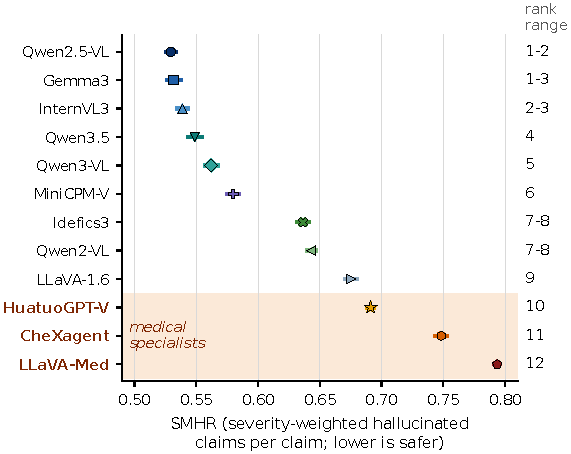
\includegraphics[width=\columnwidth]{paper_figures/fig02_smhr_ranking.pdf}
  \caption{\SMHR{} of 12 VLMs on 3,500 images (11,750 responses per model); lower is safer, and domain-adapted models are shaded. Bars are 95\% image-level bootstrap intervals (2,000 resamples, seed 42). The right-hand column gives the 95\% bootstrap range of each model's rank, so that models with overlapping ranges are not ordered.}
  \label{fig:ranking}
\end{figure}

The data support a coarse ordering and not a strict one. Of the 66 pairs of models, 63 have a paired difference whose interval excludes zero. The three exceptions are adjacent pairs: Qwen2.5-VL and Gemma3 (difference \PH{0.002}, interval \PH{$-0.006$ to $0.011$}), Gemma3 and InternVL3 (\PH{0.007}, \PH{$-0.002$ to $0.016$}) and Idefics3 and Qwen2-VL (\PH{0.007}, \PH{$-0.001$ to $0.015$}). Among the five leading models, the ten pairwise differences were tested with Holm correction. Qwen3-VL was separated from each of the other four, and Qwen3.5 was separated from Qwen2.5-VL and Gemma3 but not from InternVL3. Qwen2.5-VL, Gemma3 and InternVL3 were not separated from one another after correction. Qwen2.5-VL held the first rank in \PH{69\%} of resamples and Gemma3 in \PH{31\%}. An ordering within the first three models is therefore not supported, and the statement that can be made is that five general-purpose models formed the lowest group. Without the radiology images, Qwen2.5-VL ranked first (\SMHR{} \PH{0.428}) and Gemma3 fell to the fifth place \rad{}, which is a further reason not to rank within this group.

The \CHR{} ranged from \PH{0.715} to \PH{0.806} across models and was not correlated with the rank by \SMHR{} (Spearman $\rho = \PH{0.00}$). MiniCPM-V and CheXagent had the lowest \CHR{}, but the three lowest values (\PH{0.715} to \PH{0.730}) lie within sampling error of one another. The two metrics therefore answer different questions: the \CHR{} reports how often a response contains at least one fabrication or omission, whereas \SMHR{} reports the severity-weighted share of all claims. The number of claims extracted differs by a factor of about \PH{3.6} between models, from \PH{21,767} for LLaVA-Med to \PH{78,744} for Qwen3.5. Because \SMHR{} is a mean over claims, a model whose responses contain many correct claims can obtain a lower value without producing fewer serious errors, and the claim counts should be considered when the values are interpreted. The retrieval experiments in Section~\ref{subsec:res_mitigation} illustrate this effect.

Among the domain-adapted models, CheXagent and LLaVA-Med had the two highest \SMHR{} in every analysis. HuatuoGPT-Vision ranked tenth overall and eighth without the radiology images \rad{}, ahead of LLaVA-1.6 and Idefics3 in that analysis. The statement that the three domain-adapted models are the three worst models therefore does not hold in all analyses. It held in \PH{84\%} of random perturbations of the class weights by up to 30\%. The values for LLaVA-Med were obtained from responses of which a substantial share were truncated by a decoding defect; this is discussed in Section~\ref{subsec:res_sri}.

\subsection{Domain-adapted and general-purpose models}
\label{subsec:res_sri}

Figure~\ref{fig:sri} and Table~\ref{tab:sri} report the \SRI{} of each domain-adapted model in each modality. The reference is the general-purpose model with the lowest \SMHR{} in the modality and is held fixed in the bootstrap. It is MiniCPM-V for radiology, Qwen2.5-VL for dermatology, and Qwen3.5 for histopathology and ophthalmology. In ophthalmology Qwen3.5 (\PH{0.416}) and Qwen3-VL (\PH{0.418}) are not distinguishable, and Qwen3.5 had the lowest value in \PH{60\%} of resamples.

\begin{table}[t]
\centering
\small
\caption{Specialisation ratio index (\SRI) of the domain-adapted models, with 95\% image-level bootstrap intervals (2,000 resamples, reference model held fixed). A value above 1 indicates a higher \SMHR{} than the best general-purpose model in the modality. All twelve intervals exclude 1.}
\label{tab:sri}
\begin{tabular}{@{}lcccc@{}}
\toprule
Model & Radiology \rad{} & Dermatology & Histopathology & Ophthalmology \\
\midrule
HuatuoGPT-Vision & 1.34 [1.32, 1.36] & 1.65 [1.60, 1.70] & 1.31 [1.26, 1.37] & 1.36 [1.31, 1.41] \\
CheXagent & 1.34 [1.31, 1.36] & 1.81 [1.75, 1.87] & 1.53 [1.46, 1.59] & 1.75 [1.67, 1.82] \\
LLaVA-Med & 1.49 [1.47, 1.51] & 1.85 [1.80, 1.91] & 1.54 [1.49, 1.60] & 1.61 [1.55, 1.67] \\
\midrule
Reference model & MiniCPM-V & Qwen2.5-VL & Qwen3.5 & Qwen3.5 \\
\bottomrule
\end{tabular}
\end{table}

\begin{figure}[t]
  \centering
  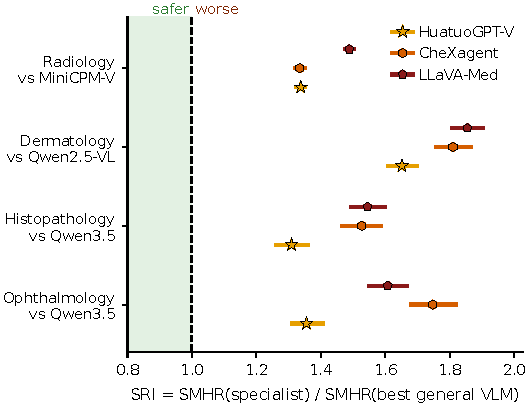
\includegraphics[width=\columnwidth]{paper_figures/fig04_specialization_paradox.pdf}
  \caption{\SRI{} of each domain-adapted model by modality. Values above 1 indicate that the model hallucinates more than the best general-purpose model named under each modality. Bars are 95\% image-level bootstrap intervals (2,000 resamples; reference model held fixed) over 3,500 images (1,200, 900, 800 and 600 per modality). The intervals of the three models overlap in several cells, and the models should not be ranked against each other from this figure.}
  \label{fig:sri}
\end{figure}

Each domain-adapted model had a higher \SMHR{} than the best general-purpose model in each of the four modalities. The \SRI{} ranged from \PH{1.31} to \PH{1.85}, the lowest lower bound of an interval was \PH{1.26}, and all twelve cells remained significant after Holm correction (adjusted $p = \PH{0.011}$, the smallest value attainable with the number of permutations used). The result was stable under the following changes.
\begin{itemize}
  \item Equal class weights: \SRI{} from \PH{1.30} to \PH{1.62}, with the lowest lower bound \PH{1.27}.
  \item Random perturbation of each class weight by up to 30\%, 2,000 draws: all twelve cells remained above 1 in every draw, with a minimum of \PH{1.13}.
  \item Selection of the reference model on one random half of the images and measurement on the other half, 1,000 splits: all twelve cells remained above 1 in every split.
  \item Removal of the radiology images: the nine remaining cells are unchanged. On the \PH{113} radiology images with distinct content the \SRI{} ranged from \PH{1.48} to \PH{1.77} \rad{}.
  \item Random flips of up to \PH{13\%} of the claim-level judge labels: all twelve cells remained above 1.
\end{itemize}

The result is a comparison of each domain-adapted model with the best of nine general-purpose models. It does not show that the domain-adapted models are worse than every general-purpose model. HuatuoGPT-Vision had a lower \SMHR{} than \PH{one} general-purpose model in radiology and in dermatology and than \PH{three} in histopathology and in ophthalmology; CheXagent had a lower \SMHR{} than one general-purpose model in radiology and than none in the other modalities; LLaVA-Med had a lower \SMHR{} than none. The comparison also does not isolate the effect of medical adaptation. The three domain-adapted models differ from the general-purpose models in parameter count, in architecture and in the date of release, and the design contains no base--specialist pairs. CheXagent was developed for chest radiography, so that its values in the other three modalities measure in part the transfer of a chest radiograph model to other domains. The ratio of \SMHR{} to the reference should therefore be read as a descriptive measurement for the checkpoints and the protocol examined here.

The \SRI{} of LLaVA-Med is an upper bound. In the core run, a decoding defect caused \PH{about one third} of the LLaVA-Med responses to begin in mid-sentence.
% NOTE: the audit gives 32% of responses; figure_manifest.md gives 50% of Q1 responses. State the basis of the percentage. On the responses that were regenerated with the corrected decoder the \SMHR{} was \PH{0.728}, against \PH{0.791} for the same items in the core run, a reduction of about \PH{8\%}. The \SRI{} values of LLaVA-Med stay above 1 under this correction.
% NOTE: confirm whether the core run is rerun or both numbers are reported; the core-run numbers are the ones in T3.

\subsection{Dependence on modality, image type and query}
\label{subsec:res_modality}

Figure~\ref{fig:modality} shows the \SMHR{} of each model in each modality and the composition of the flagged claims by class. Radiology had the highest \SMHR{} for 10 of the 12 models, and this held also on the \PH{113} radiology images with distinct content \rad{}. Dermatology had the lowest \SMHR{} for 9 of the 12 models, with a bootstrap range of 6 to 10 models. Modality and model identity each accounted for roughly 40\% to 50\% of the variance in the 48 cell-level values of \SMHR{}. This is a descriptive decomposition of the cells and not a test.

\begin{figure*}[t]
  \centering
  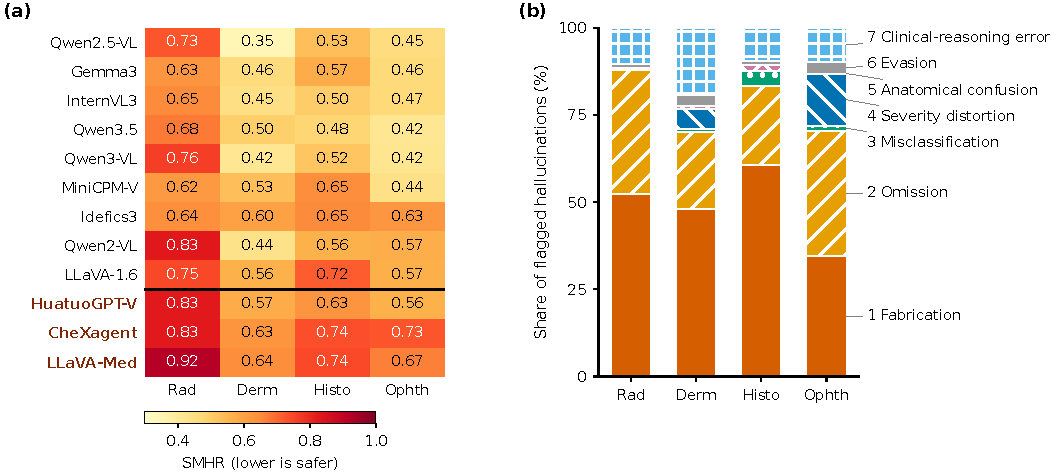
\includegraphics[width=\textwidth]{paper_figures/fig03_modality_fingerprints.pdf}
  \caption{(a) \SMHR{} by model and modality; the intervals of each cell are given in the source data. (b) Share of flagged claims by hallucination class within each modality, pooled over the 12 models (353,625 flagged claims and omissions). The thick line separates general-purpose models (above) from domain-adapted models (below).}
  \label{fig:modality}
\end{figure*}

The composition of errors differs between modalities. Fabrication and omission together accounted for \PH{88\%} of the flagged claims in radiology \rad{}, \PH{83\%} in histopathology, \PH{71\%} in ophthalmology and \PH{70\%} in dermatology. Fabrication was the largest class in radiology, dermatology and histopathology (\PH{52\%}, \PH{48\%} and \PH{61\%}), and omission was the largest in ophthalmology (\PH{36\%}). Clinical reasoning error accounted for \PH{19\%} of the flagged claims in dermatology and \PH{10\%} in each of the other modalities, and severity distortion for \PH{15\%} in ophthalmology and \PH{6\%} in dermatology. Anatomical confusion, evasion and misclassification each accounted for no more than \PH{5\%} in any modality. The class-specific labels are not validated against independent annotation (Section~\ref{sec:validation}), so that this composition is descriptive.

The interpretation of the \SMHR{} depends on how much of each class can be checked against the available ground truth. In radiology, \PH{93\%} of the weighted error comes from classes with full coverage by the labels, although the radiology labels are subject to the image issue \rad{}. In dermatology the share is \PH{57\%}, in ophthalmology \PH{50\%}, and in histopathology none, because essentially all of the weighted error (\PH{99.9\%}) comes from classes that can be checked only partially, fabrication and omission alone accounting for \PH{89\%}: the PatchCamelyon half of the histopathology images has binary tumour labels only. The \SMHR{} in histopathology is therefore a proxy for the hallucination rate and not a complete measurement of it.

Normal images did not uniformly draw more hallucination than abnormal ones. Across the four modalities and twelve models, the difference in \SMHR{} between the normal and the abnormal strata for the first three queries had either sign, with the exception of ophthalmology, where the \SMHR{} on normal images was lower for all twelve models (mean difference \PH{$-0.31$}). The false-premise query had a clear effect on normal images. The \SMHR{} for the fourth query was higher than for the first three queries for \PH{10 of the 12} models, lower for one (Qwen3-VL) and unchanged for one (HuatuoGPT-Vision), with a mean difference of \PH{0.14}. Figure~\ref{fig:normal} in the appendix gives the underlying values. This differs from the finding of HalluCXR that normal radiographs drew the most severe hallucinations \citep{wang2026hallucxr}, which was obtained for chest radiographs only and with a different grading scheme, and the present data do not permit a direct comparison.

\subsection{Agreement of rankings across modalities}
\label{subsec:res_transfer}

The rankings of the twelve models by \SMHR{} in dermatology, histopathology and ophthalmology were positively correlated (Figure~\ref{fig:transfer} in the appendix). The Spearman correlation was \PH{0.81} for dermatology and histopathology (permutation $p = \PH{0.002}$, Holm-adjusted $p = \PH{0.013}$), \PH{0.77} for histopathology and ophthalmology (\PH{0.005}, \PH{0.024}) and \PH{0.66} for dermatology and ophthalmology (\PH{0.022}, \PH{0.088}). The last of these does not remain significant after correction. Among the nine general-purpose models alone the correlations were smaller and none was significant (\PH{0.62}, \PH{0.60} and \PH{0.33}). The cross-modality association therefore reflects in large part the fact that the domain-adapted models and the weakest general-purpose models rank poorly in every modality. With three domain-adapted models, a correlation of the \SRI{} values across modalities cannot reach a two-sided $p$ below \PH{0.33}, and it is not reported.

The correlations between radiology and the other modalities were \PH{0.21}, \PH{0.27} and \PH{0.49}, none of them significant. On the \PH{113} radiology images with distinct content they were \PH{0.36}, \PH{0.55} and \PH{0.69}. The first set is an artefact of the duplicated images, and the second rests on a small number of images. Whether rankings transfer to and from radiology could not be assessed in this study \rad{}.
% NOTE: Fig 6 labels its Holm p-values from a t-based test (0.008, 0.074, 0.017); the audit uses permutation p-values (0.013, 0.088, 0.024). Use one convention.

\subsection{Comparison with published scores}
\label{subsec:res_metrics}

The \SMHR{} was compared with the risk-weighted score of CREST \citep{crest2025medrxiv} and with the MediHall Score \citep{chen2024medhallmark}, both computed on the same classified claims. The comparison is shown in Figure~\ref{fig:concordance} in the appendix. The \SMHR{} and CREST were positively rank-correlated across the twelve models (Spearman $\rho = \PH{0.64}$, permutation $p = \PH{0.03}$, 95\% interval \PH{0.07 to 0.90} by Fisher transformation). The CREST values were confined to a narrow interval (\PH{2.67 to 2.86} on a scale from 1 to 3), so that the agreement rests on small differences. Seven of ten model--modality cells in which the two scores diverge by more than one standard deviation were stable in more than \PH{90\%} of the bootstrap resamples, and three lay at the threshold. The \SMHR{} and the MediHall Score ranked the twelve models identically ($\rho = \PH{-1.00}$). This agreement is expected from the construction of the two scores, since both are weighted error rates over the same classified claims and their class weights correlate with $r = \PH{0.95}$, and it should not be read as independent confirmation. The unweighted error rate alone correlates with the \SMHR{} at $\rho = \PH{0.965}$. On these data the \SMHR{} therefore does not order the models differently from a MediHall-style score. Its distinct contributions are the claim as the unit of analysis, the explicit omission class, and the cross-modality reference provided by the \SRI{}.

\subsection{Robustness}
\label{subsec:res_robust}

Three sources of uncertainty not captured by the image-level bootstrap were examined.

\paragraph{Class weights.} Under equal weights and under 200 random perturbations of up to 30\% the ranking of the twelve models was essentially unchanged (Spearman $\rho \geq \PH{0.88}$ against the ranking with the assumed weights). The weights themselves were not elicited from clinicians, so that this analysis establishes only the stability of the conclusions with respect to the weights.

\paragraph{Judge labels.} All values depend on one local model that extracts and judges claims (Section~\ref{sec:setup}). The only component independent of this model is the omission count of the first layer, which accounts for between \PH{25\%} and \PH{42\%} of the weighted error. Re-running the judge on identical text changed \PH{1.1\%} of the strict and \PH{2.8\%} of the claim-level labels, and the labels produced by the core pipeline and by the later pipeline for the same responses differed for \PH{2.1\%} and \PH{11.3\%} of \PH{195} responses. Symmetric random flips of 3\% and 5\% of the claim-level labels changed none of the main conclusions. At 13\% the identity of the two leading models changed. Systematic bias of the judge, for example towards outputs of models of the same family, was not assessed, and the evaluated set contains four models of the Qwen family.

\paragraph{Sampling.} The core run used one sample per image and query at temperature 0.1. Across four distinct decoding settings, the \SMHR{} of a single model varied by between \PH{0.022} (Qwen2.5-VL) and \PH{0.077} (HuatuoGPT-Vision), which exceeds the differences of \PH{0.002} to \PH{0.010} within the first three models. Stochasticity can therefore change the order within the leading group. It cannot remove the gap of \PH{0.13} to \PH{0.26} between the five leading models and the domain-adapted models.

\subsection{Mitigation}
\label{subsec:res_mitigation}

Two inference-time strategies were compared on a subset of 500 images and five models: retrieval-augmented prompting and contrastive decoding. Fine-tuning was planned and not carried out. Both strategies were run with greedy decoding. The benchmark baseline is the response from the core run, generated by sampling at temperature 0.1. Because a change from sampling to greedy decoding can alter \SMHR{} by itself, each strategy is also compared with a matched greedy baseline from the calibration experiment. The matched baseline exists only for the items on which the greedy response stated a confidence, which is \PH{1,489}, \PH{1,179}, \PH{1,499} and \PH{1,385} of about 1,670 items for Qwen2.5-VL, LLaVA-1.6, CheXagent and HuatuoGPT-Vision, respectively; for LLaVA-Med the corrected greedy rerun was used. Decoding alone moved the \SMHR{} of LLaVA-1.6 by \PH{$-0.046$}, an interval excluding zero, and that of Qwen2.5-VL by \PH{$-0.011$}.

\begin{table*}[t]
\centering
\footnotesize
\caption{Change in \SMHR{} under retrieval-augmented prompting (RAG) and contrastive decoding (CD) on a 500-image subset, against the benchmark baseline (temperature 0.1) and a matched greedy baseline. Entries are the difference [95\% paired image-level bootstrap interval], with the Holm-adjusted $p$-value in parentheses (families of 10 tests per baseline). $^{\dagger}$ domain-adapted model. The subset includes radiology images affected by the image issue \rad{}.}
\label{tab:mitigation}
\begin{tabular}{@{}lcccc@{}}
\toprule
& \multicolumn{2}{c}{RAG} & \multicolumn{2}{c}{CD} \\
\cmidrule(lr){2-3}\cmidrule(lr){4-5}
Model & vs benchmark & vs matched greedy & vs benchmark & vs matched greedy \\
\midrule
Qwen2.5-VL & $-0.028$ [$-0.046$, $-0.011$] (0.015) & $-0.018$ [$-0.034$, $-0.001$] (0.26) & $-0.003$ [$-0.021$, $+0.016$] (1.00) & $+0.009$ [$-0.009$, $+0.027$] (1.00) \\
LLaVA-1.6 & $-0.042$ [$-0.061$, $-0.021$] (0.003) & $+0.041$ [$+0.021$, $+0.060$] (0.010) & $-0.085$ [$-0.105$, $-0.065$] (0.001) & $-0.031$ [$-0.053$, $-0.008$] (0.048) \\
HuatuoGPT-V$^{\dagger}$ & $+0.004$ [$-0.011$, $+0.019$] (1.00) & $-0.011$ [$-0.028$, $+0.005$] (0.96) & $-0.025$ [$-0.040$, $-0.010$] (0.015) & $-0.035$ [$-0.051$, $-0.020$] (0.001) \\
CheXagent$^{\dagger}$ & $+0.026$ [$+0.005$, $+0.048$] (0.12) & $+0.011$ [$-0.013$, $+0.035$] (1.00) & $-0.041$ [$-0.068$, $-0.015$] (0.028) & $-0.052$ [$-0.081$, $-0.022$] (0.010) \\
LLaVA-Med$^{\dagger}$ & $+0.003$ [$-0.010$, $+0.014$] (1.00) & $+0.003$ [$-0.010$, $+0.014$] (1.00) & $-0.005$ [$-0.019$, $+0.009$] (1.00) & $-0.005$ [$-0.019$, $+0.009$] (1.00) \\
\bottomrule
\end{tabular}
\end{table*}

Table~\ref{tab:mitigation} gives the results. Contrastive decoding gave the lowest \SMHR{} for four of the five models, and the reduction was reliable against the matched baseline for three of them: CheXagent ($-0.052$), HuatuoGPT-Vision ($-0.035$) and LLaVA-1.6 ($-0.031$). For LLaVA-Med and Qwen2.5-VL it was indistinguishable from the baseline. The reduction for HuatuoGPT-Vision was the only effect that held against both baselines and with and without the radiology images ($-0.025$ against the benchmark baseline and $-0.035$ against the matched baseline; $-0.050$ and $-0.062$ without radiology \rad{}). Without radiology, contrastive decoding increased the \SMHR{} of CheXagent by \PH{0.048} to \PH{0.056} (Holm-adjusted $p = \PH{0.05}$ to \PH{0.08}), so that its benefit for this model depends on the radiology images \rad{}.

Retrieval-augmented prompting did not lower \SMHR{} consistently. Against the benchmark baseline it appeared to lower it for Qwen2.5-VL and LLaVA-1.6, but against the matched greedy baseline the change for Qwen2.5-VL was not significant after correction, and for LLaVA-1.6 the \SMHR{} was higher by \PH{0.041}. The apparent gain for LLaVA-1.6 was concentrated in items on which the greedy response states no confidence and for which no matched label exists. On exactly the items that have one, the effect against the benchmark baseline was \PH{$-0.006$} [\PH{$-0.027$}, \PH{$+0.016$}]. For CheXagent the increase against the benchmark baseline was not significant after correction. Without the radiology images, retrieval increased the \SMHR{} of LLaVA-Med by \PH{0.037} (Holm-adjusted $p = \PH{0.010}$) \rad{}. In a direct comparison, contrastive decoding gave a lower \SMHR{} than retrieval for LLaVA-1.6, CheXagent and HuatuoGPT-Vision (Holm-adjusted $p \leq \PH{0.002}$), retrieval gave a lower value for Qwen2.5-VL ($+0.025$ in favour of retrieval, $p = \PH{0.015}$), and the two were tied for LLaVA-Med.

The \SMHR{} does not capture a second effect of retrieval. The share of responses that contain a fabrication or omission (\CHR{}) increased under retrieval for four of the five models: by \PH{0.12} for LLaVA-1.6, \PH{0.08} for HuatuoGPT-Vision, \PH{0.05} for CheXagent and \PH{0.03} for LLaVA-Med, with all four intervals excluding zero. For Qwen2.5-VL the increase of \PH{0.020} [\PH{$-0.003$}, \PH{$+0.042$}] was not distinguishable from zero. Retrieved text lengthened the answers and added correct claims, which can leave the \SMHR{} flat or lower it while more responses contain at least one serious error. A decrease in \SMHR{} under retrieval should not be read as a decrease in the number of harmful responses.

For the specialisation analysis, the mean \SRI{} over the twelve cells was \PH{1.401} for the benchmark baseline, \PH{1.516} for the matched greedy baseline, \PH{1.474} with retrieval and \PH{1.406} with contrastive decoding. Contrastive decoding reduced the mean \SRI{} against the matched greedy baseline by \PH{0.110} [\PH{0.039}, \PH{0.183}], and it did not change it against the benchmark baseline. Retrieval did not detectably change it. Neither strategy removed the gap between domain-adapted and general-purpose models.

\begin{figure}[t]
  \centering
  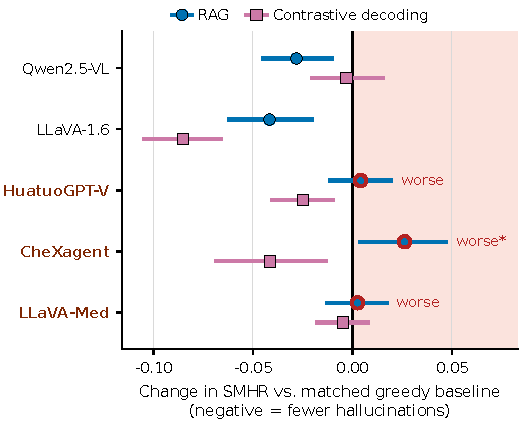
\includegraphics[width=\columnwidth]{paper_figures/fig09_mitigation.pdf}
  \caption{Change in \SMHR{} relative to the benchmark baseline for retrieval-augmented prompting and contrastive decoding (five models, 1,659 to 1,678 paired image--query responses on a 500-image subset). Bars are 95\% paired image-level bootstrap intervals (2,000 resamples). Outlines mark strategies that increase \SMHR{}.}
  \label{fig:mitigation}
\end{figure}
% NOTE: Fig 9 and T4 were produced against the benchmark baseline; the manifest caption calls it a matched greedy baseline, which is incorrect. Regenerate Fig 9 against the matched greedy baseline, or keep this caption.

\subsection{Calibration of stated confidence}
\label{subsec:res_calibration}

The calibration of stated confidence was examined for five models under six decoding configurations on the same subset (Figure~\ref{fig:calibration} in the appendix). Under the strict correctness label, accuracy was between \PH{12\%} and \PH{28\%} while the mean stated confidence was between \PH{52\%} and \PH{91\%}. The expected calibration error was between \PH{0.50} and \PH{0.73}, and at least \PH{75\%} of the gap came from overconfident bins. The three greedy configurations produced identical responses, so that four configurations are independent. Across these four, the ordering of the five models by calibration error was stable (mean pairwise Spearman $\rho = \PH{0.90}$, 95\% interval \PH{0.83 to 0.95}, with the image as the unit of resampling), and HuatuoGPT-Vision was the worst-calibrated model in every configuration. With one prompt and five models, this result shows that the ordering is insensitive to the decoding setting. It does not show that calibration is a property of the model weights.

% ===================== sec_validation.tex =====================
% NOTE: sources: annotation_report.md, annotation_paper_paragraphs.tex, paper_tables/T5_annotation_agreement.tex, figure_manifest.md (Fig 12), claim_audit_report.md (X2, Check 4). The text follows Version B of the validation design: the annotators are language-model personas, and no claim of clinician validation is made. If real clinician annotations are obtained, this section must be rewritten.
% NOTE: the annotation files were committed first as ai_annotations/ and later renamed human_annotations/ (claim_audit_report.md, X2). State in the covering letter or the data statement that the set is simulated.
\section{Audit of the Labelling Pipeline}\label{sec:validation}

Every value in Section~\ref{sec:results} rests on one pipeline that extracts claims and classifies them (Section~\ref{sec:pipeline}). This section reports an audit of the labels that the pipeline assigns. The audit has a narrow scope. No clinician has annotated any part of the benchmark. The only independent annotation available is a set produced by six simulated annotators, and the audit therefore tests whether the pipeline agrees with an independent panel of language-model annotators. It does not test whether the pipeline agrees with the judgement of clinicians.

\subsection{Annotation set}\label{sec:val_set}
The set contains 720 generated texts, 180 for each modality. They are the responses of five models (Qwen2.5-VL, LLaVA-1.6, CheXagent, HuatuoGPT-Vision and LLaVA-Med) under the three conditions of the mitigation experiment (benchmark response, retrieval-augmented prompting and contrastive decoding), for 48 images, which are three for each combination of modality and query type. Each text was rated by six simulated annotators, which are a language model other than the pipeline judge prompted to act in six roles: a generalist, four modality specialists (radiology, dermatology, histopathology and ophthalmology) and an undergraduate student. Each annotator gave six scores on a scale from 0 to 5 (factual correctness, completeness, clinical safety, informativeness, clarity and overall quality) and flagged each of the seven hallucination classes as present or absent. The annotators are called simulated throughout, and the roles describe the instruction that each was given and not a qualification that any of them holds.
% NOTE: state which language model produced the annotations and the exact role prompts, or place them in the appendix.

Two properties of the set limit what it can show. First, the 720 texts rest on 48 images, with 15 texts for each image, so that the texts are clustered. Intervals in this section resample texts as if they were independent and are therefore too narrow. Second, \rad{the 12 radiology images are all the same file (Section~\ref{sec:data}), so that the radiology part of the set contains one radiograph}.

\subsection{Agreement among the simulated annotators}\label{sec:val_agree}
Table~\ref{tab:annotation} gives the agreement. The six annotators agree closely on the scores. The single-rater intraclass correlation, ICC(2,1), lies between \PH{0.829} for clinical safety and \PH{0.926} for clarity. The ICC for the mean of six raters is at least \PH{0.967}, and this value is high by construction in a fully crossed design with six raters. The agreement on the class flags is lower and depends on the class. The Fleiss $\kappa$ is \PH{0.70} for fabrication and \PH{0.78} for evasion, \PH{0.50} to \PH{0.51} for misclassification and severity distortion, and \PH{0.41}, \PH{0.36} and \PH{0.36} for omission, anatomical confusion and clinical reasoning error. Anatomical confusion was flagged for \PH{5\%} of the ratings, so that its $\kappa$ is unstable. Annotators in a specialist role did not agree more with the others on their own modality than on another one: for factual correctness the ICC of pairs formed by a specialist on the own modality and a non-specialist was \PH{0.853} [\PH{0.829}, \PH{0.872}], against \PH{0.864} [\PH{0.841}, \PH{0.881}] for pairs of specialists of other modalities.

These values describe the consistency of a set of language-model annotators and they should not be read as the reliability of human readers. The six annotators are driven by one generator and share its tendencies, so that agreement among them is expected to be higher than agreement among independent persons. The annotators also rated the texts severely, with a mean factual-correctness score of \PH{1.1} to \PH{2.2} on the scale of 5 depending on annotator and modality, and flagged at least one class for \PH{87\%} of the texts. Both properties lower $\kappa$ and raise raw agreement.

\begin{table}[t]
\centering
\small
\begin{tabular}{lcccc}
\toprule
Score (0--5) & ICC(2,1) [95\% CI] & ICC(2,k) & Alpha & QWK \\
\midrule
factual correctness & 0.860 [0.842, 0.877] & 0.974 & 0.860 & 0.845 \\
completeness & 0.863 [0.845, 0.881] & 0.974 & 0.863 & 0.842 \\
clinical safety & 0.829 [0.809, 0.847] & 0.967 & 0.829 & 0.812 \\
informativeness & 0.858 [0.840, 0.874] & 0.973 & 0.857 & 0.840 \\
clarity & 0.926 [0.914, 0.937] & 0.987 & 0.926 & 0.915 \\
overall & 0.877 [0.860, 0.892] & 0.977 & 0.877 & 0.862 \\
\bottomrule
\end{tabular}
\par\medskip
\small
\begin{tabular}{lcccc}
\toprule
Hallucination class & Prevalence & Fleiss $\kappa$ [95\% CI] & Judge vs. majority $\kappa$ [95\% CI] & Judge F1 \\
\midrule
Fabrication & 0.59 & 0.70 [0.66, 0.73] & 0.40 [0.34, 0.47] & 0.74 \\
Omission & 0.26 & 0.41 [0.37, 0.44] & 0.18 [0.12, 0.24] & 0.51 \\
Misclassification & 0.35 & 0.50 [0.46, 0.54] & 0.04 [0.00, 0.08] & 0.10 \\
Severity distortion & 0.40 & 0.51 [0.48, 0.55] & 0.11 [0.05, 0.17] & 0.30 \\
Anatomical confusion$^{a}$ & 0.05 & 0.36 [0.28, 0.43] & -0.01 [-0.02, -0.01] & undef. \\
Evasion & 0.20 & 0.78 [0.74, 0.81] & -0.06 [-0.09, -0.03] & 0.01 \\
Clinical reasoning error & 0.10 & 0.36 [0.30, 0.42] & 0.15 [0.08, 0.23] & 0.25 \\
\bottomrule
\end{tabular}
\caption{Agreement among six \emph{simulated (AI-persona) annotators} on 720 items (48 distinct images), and between the LLM judge and the annotator majority. No clinician annotations are included. Intervals are 95\% item-level bootstrap CIs and are optimistic because items share images; $^{a}$ rare class, $\kappa$ unstable.}
\label{tab:annotation}
\end{table}


\begin{figure*}[t]
  \centering
  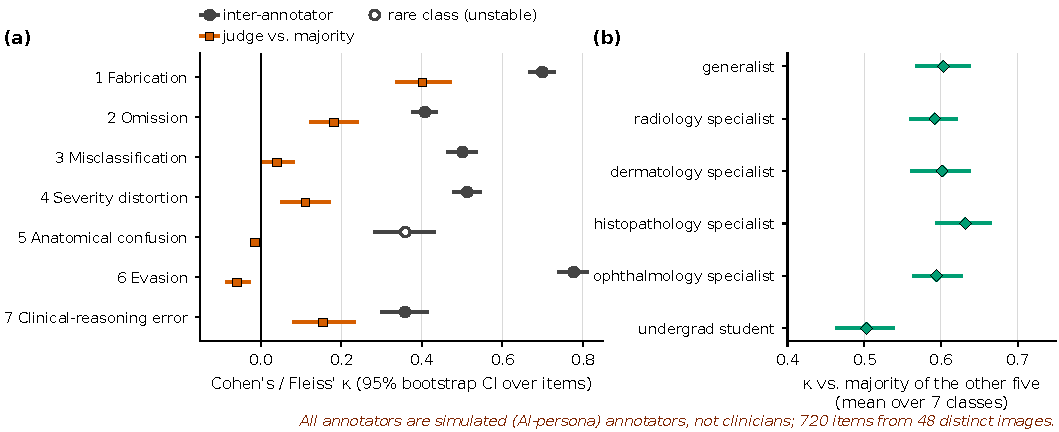
\includegraphics[width=\textwidth]{paper_figures/fig12_annotation_agreement.pdf}
  \caption{(a) Agreement per hallucination class among the six simulated annotators (Fleiss $\kappa$) and between the language-model judge and their majority label (Cohen $\kappa$), for 720 texts from 48 images. (b) Mean $\kappa$ of each annotator with the majority of the other five. Bars are 95\% bootstrap intervals over texts (2{,}000 resamples), which are too narrow because texts share images. No clinician annotation is included.}
  \label{fig:annotation}
\end{figure*}

\subsection{Agreement of the pipeline with the annotator majority}\label{sec:val_judge}
The pipeline was compared with the majority of the simulated annotators. A class is positive for a text if at least four of the six annotators flag it, and a tie of three against three is resolved by the annotator in the role of specialist for the modality of the text. The annotators flag classes for a whole text, so the comparison is made at the level of the text. The claim-level output of the pipeline is aggregated by marking a class as present if any claim is assigned to it, and the omissions of Layer 1 are counted in the omission class, as in the definition of the \SMHR{}. Three of the 720 texts have no usable pipeline label, which leaves 717.

\paragraph{Any hallucination.} The combined label of the pipeline, positive when any class is present, reached a precision of \PH{0.888}, a recall of \PH{0.901} and an $F_1$ of \PH{0.895} [\PH{0.877}, \PH{0.912}] against the majority label. The threshold of 0.90 set in the study protocol was therefore not met at the point estimate, and the interval spans it. The thresholds set for the layers taken separately (0.95 for Layer 1 and 0.90 for Layer 2) were not met either; the layer-wise comparisons use the label for all classes and are indicative. By modality, the $F_1$ of the combined label was \PH{0.971} [\PH{0.950}, \PH{0.986}] in radiography \rad{(one radiograph)}, \PH{0.841} [\PH{0.795}, \PH{0.886}] in dermoscopy, \PH{0.903} [\PH{0.867}, \PH{0.936}] in histopathology and \PH{0.848} [\PH{0.803}, \PH{0.888}] in fundus photography.

This $F_1$ is not good evidence of discrimination. The annotators flagged at least one class for \PH{626} of the \PH{717} texts, which is \PH{87\%}, and a rule that flags every text would reach a precision of \PH{0.873}, a recall of 1 and an $F_1$ of \PH{0.932}, higher than the value of the pipeline. The Cohen $\kappa$ of the combined label with the majority is \PH{0.126}, which indicates only slight agreement beyond chance. At this prevalence the $F_1$ for the presence of any hallucination cannot separate a labelling pipeline from a rule that always reports a hallucination, and the audit does not support a claim of validation at this level.

\paragraph{Individual classes.} Class-level agreement is weaker (Table~\ref{tab:annotation} and Figure~\ref{fig:annotation}). Fabrication is the class that the pipeline reproduces best, with a precision of \PH{0.767}, a recall of \PH{0.714}, an $F_1$ of \PH{0.74} and a $\kappa$ of \PH{0.40} [\PH{0.34}, \PH{0.47}]. Omission is over-called, with a precision of \PH{0.385} and a recall of \PH{0.751} ($F_1$ \PH{0.51}, $\kappa$ \PH{0.18}). The pipeline rarely assigns misclassification, severity distortion or evasion, which the annotators flag often; its recall for them is \PH{0.053}, \PH{0.206} and \PH{0.007}. For anatomical confusion, the pipeline found none of the \PH{30} texts that the majority flagged. For clinical reasoning error the pipeline flags \PH{153} texts against \PH{51} for the majority, with a precision of \PH{0.163}. The class that the pipeline regards as the most severe in a text agrees with that of the majority for \PH{55\%} of the texts.

Two differences between the methods qualify these figures. The annotators judge a text as a whole against their own reading of the case, while the pipeline compares claims with the reference labels, which record only a subset of the findings in an image, so that the two do not define omission or evasion in the same way. Differences between them therefore do not show which of the two is closer to the intended meaning of a class. The values nevertheless establish that the class-specific labels of the pipeline cannot be described as validated, and the class composition reported in Section~\ref{subsec:res_modality} is descriptive only.

\subsection{Relation to the item-level \SMHR{}}\label{sec:val_smhr}
A weaker check does not depend on the class flags. For each text with at least one claim, the mean factual-correctness score of the annotators was correlated with the \SMHR{} of the text. The Spearman correlation was \PH{$-0.31$} [\PH{$-0.38$}, \PH{$-0.23$}] for \PH{682} texts, in the expected direction and of moderate size. It was \PH{$-0.47$} in dermoscopy, \PH{$-0.34$} in fundus photography and \PH{$-0.20$} in radiography \rad{}, and the interval included zero in histopathology (\PH{$-0.08$} [\PH{$-0.24$}, \PH{0.08}]). A moderate correlation is the size that is expected between a holistic rating and a ratio of weighted claims. At the level of the model, the rank correlation between the mean factual-correctness score of each annotator and the \SMHR{} was \PH{$-0.7$} for the five models, which is moderate and rests on five points.

\subsection{What the audit supports}\label{sec:val_summary}
The audit supports three statements. The pipeline agrees moderately with an independent panel of language-model annotators for the presence of fabrication, and weakly for most other classes. Its text-level \SMHR{} is moderately and negatively related to the factual-correctness ratings of the panel. The ranking of the models and the comparison of domain-adapted and general-purpose models do not depend on the class weights within the ranges tested (Section~\ref{subsec:res_robust}). The audit does not support the statements that clinicians would agree with the labels, that the class weights reflect clinical harm, or that the class-specific labels are valid. Agreement with an independent language-model panel is weaker evidence than agreement with clinicians, because the panel and the judge may share errors of a kind that readers of images would not make.

% ===================== sec_discussion.tex =====================
% NOTE: every sentence in this section interprets a result reported in Sections 5 and 6. Explanations that were not tested are written as hypotheses and are marked as such. No causal wording is used for observational comparisons (claim_audit_report.md, Check 9).
\section{Discussion}\label{sec:discussion}

\subsection{Principal findings}\label{sec:disc_findings}
Four findings emerge from the evaluation of twelve models on four imaging modalities. First, five general-purpose models formed the group with the lowest \SMHR{}, and the data do not support an order within the three leading models. A coarse ordering is therefore the most that this benchmark can offer, and a single best model should not be named from it. Second, each of the three domain-adapted models had a higher \SMHR{} than the best general-purpose model in every modality, by a factor of \PH{1.31} to \PH{1.85}. This result remained under equal class weights, under random changes of the weights, under selection of the reference model on half of the images and under symmetric noise in the judge labels. Third, the level of \SMHR{} depends strongly on the modality, with the highest values in radiography \rad{} and the lowest in dermoscopy, and the composition of the errors differs between modalities. Fourth, the experiments on mitigation and calibration gave results that are specific to the model and, in the case of retrieval, depend on the choice of the baseline.

The second finding is the one that bears most directly on the use of domain-adapted models, and it should be read within its limits. The comparison is with the best of nine general-purpose models, and not with all of them. One domain-adapted model, HuatuoGPT-Vision, had a lower \SMHR{} than between one and three of the general-purpose models in every modality. The three domain-adapted models differ from the general-purpose models in size, architecture and date of release, and the design contains no pair of a base model and the model adapted from it. A difference in \SMHR{} cannot therefore be attributed to the adaptation itself. Studies that did use such pairs found no reliable improvement from medical fine-tuning, with results that depended on the task and on the wording of the prompt \citep{mclaughlin2026knowledge,sabbaghziarani2026confident}, and other studies found that medical models can be less robust than general ones \citep{wu2024halluvqa,gu2024medvh,xu2025sycophancy}. The present result is consistent with these reports. It adds a measurement made with one protocol for four modalities, and it does not explain the difference.

\subsection{Possible explanations of the specialisation result}\label{sec:disc_explain}
Several explanations are compatible with the data, and none of them was tested here. We list them to indicate what the design cannot exclude.
\begin{itemize}
  \item \emph{Style of the response.} The \SMHR{} is a mean over claims. Models that produce short answers contribute fewer claims, and each error then carries more weight in the mean. The two domain-adapted models with the shortest outputs, LLaVA-Med and CheXagent, yielded \PH{21,767} and \PH{24,685} claims and omissions over \Ncalls{} responses each, against \PH{78,744} for Qwen3.5. The comparison of retrieval-augmented prompting in Section~\ref{subsec:res_mitigation} shows that the number of correct claims can move the \SMHR{} without a change in the share of responses with a serious error. The \CHR{} does not depend on the number of claims in the same way, and it ordered the domain-adapted models less unfavourably (CheXagent had one of the lowest values), which is consistent with a part of the difference arising from the length and style of the response.
  \item \emph{Mismatch of the prompts.} The queries are free-text instructions in a common format. A domain-adapted model may have been trained on data with a narrower format, for example captions, reports or multiple-choice questions, and may follow an open instruction less reliably.
  \item \emph{Quantisation and decoding.} All models were run with 4-bit quantisation and with sampling at a low temperature. The effect of quantisation may differ between models, and for LLaVA-Med a decoding defect truncated a large share of the responses (Section~\ref{subsec:res_sri}).
  \item \emph{Scope of training data.} CheXagent was developed for chest radiography, and its values in the other three modalities measure in part the transfer of a model for one modality to others. LLaVA-Med was developed for broader biomedical use, and its \SRI{} values in the other three modalities were similar to those of CheXagent, while those of HuatuoGPT-Vision were lower.
  \item \emph{Interaction with the judge.} The judge is a general-purpose language model, and a general-purpose judge may rate the typical output of a general-purpose model more favourably. The audit could not test this (Section~\ref{sec:val_summary}).
\end{itemize}
A study that settles the question requires base--specialist pairs, full-precision inference, repeated sampling and a judge from a different family, and we return to this in the final section.

\subsection{Implications for the evaluation of medical vision-language models}\label{sec:disc_eval}
\paragraph{Weighting by severity changes the interpretation more than the ranking.} The ranking of the models by \SMHR{} was nearly unchanged when the class weights were set to be equal or perturbed by up to 30\%, and it was identical to the ranking by the MediHall Score, which is a weighted error rate over the same classified claims. On these data, severity weighting therefore does not by itself reorder the models. Its value lies in what it reports: the \SMHR{} states how much of the error comes from the classes that carry the highest potential for harm, and the class composition shows that fabrication and omission account for between \PH{70\%} and \PH{88\%} of the flagged claims in the four modalities. A reader who accepts the order of the classes can interpret the score. A reader who does not can recompute it with other weights, which is possible if the class labels are released with the benchmark.

\paragraph{A rate per claim and a rate per response answer different questions.} The \SMHR{} and the \CHR{} were not correlated across models ($\rho = \PH{0.00}$), and, against the benchmark baseline, retrieval-augmented prompting lowered or left unchanged the \SMHR{} of LLaVA-1.6, HuatuoGPT-Vision and LLaVA-Med while it raised their \CHR{}. A model can add correct statements to its answer and lower the rate per claim while more of its answers contain a serious error. A benchmark that reports only a rate per claim, or only a rate per response, can be improved on the reported measure by changes that do not improve the answers. We recommend that both be reported, together with the number of claims.

\paragraph{Mitigation studies need a matched baseline.} Changing the decoding setting from sampling at a temperature of 0.1 to greedy decoding changed the \SMHR{} of LLaVA-1.6 by \PH{$-0.046$}. This is comparable in size to the apparent effects of the mitigation strategies, and it reversed the sign of the apparent benefit of retrieval for the same model. The only effect of mitigation that held against both baselines, with and without the radiology images, was the reduction in \SMHR{} for HuatuoGPT-Vision under contrastive decoding. The other effects were specific to a model, small or of uncertain sign, and the experiment does not support a general recommendation for either strategy.

\paragraph{Stated confidence is not a usable safety signal for these models.} The accuracy of the responses under the strict label was between \PH{12\%} and \PH{28\%}, while the confidence that the models stated averaged between \PH{52\%} and \PH{91\%}. The label is demanding, since a response is counted as correct only if it contains no hallucination of any class, but the gap is large for every model and configuration, and it came mostly from overconfident bins. The order of the models by calibration error varied little with the decoding setting, and HuatuoGPT-Vision was the worst-calibrated model in every configuration. With one prompt and five models, we regard this as a description of the models examined and not as a property of their weights.

\paragraph{The modality changes what the score means.} The \SMHR{} reflects different mixes of error in different modalities, and the share of the weighted error that can be checked against the reference labels varied between modalities. In histopathology, almost all of the weighted error arose from classes that could be checked only in part, because half of the patches carry a binary tumour label alone. A value of \SMHR{} in one modality is therefore not the same quantity as a value in another, and the \SRI{}, which compares models within a modality, is more interpretable across modalities than the absolute rates.

\subsection{Interpretation for clinical use}\label{sec:disc_clinical}
The metrics describe the disagreement of model statements with the reference labels, weighted by an assumed order of harm. They do not describe the harm to patients, they do not use clinical outcomes, and they do not establish that any model is safe or unsafe in practice. The reference labels are coarse, since they record a diagnosis or a small set of findings and not a complete reading of the image, and a statement that is absent from the labels is counted as unsupported even when it may be correct. The finding that the domain-adapted models had higher rates than the best general-purpose models does not imply that general-purpose models are suitable for clinical use, because the rates of the best group are themselves high (\SMHR{} from \PH{0.529}) and the proportion of responses with a fabrication or an omission was between \PH{72\%} and \PH{81\%} for all twelve models. We regard the results as evidence of the size of the problem in the models examined, and as a method for measuring it.

% ===================== sec_limitations.tex =====================
% NOTE: each paragraph corresponds to an item in claim_audit_report.md or reconcile_questions.md. Delete the paragraph on the radiology arm only if the arm is re-extracted and rerun.
\section{Limitations}\label{sec:limitations}

\paragraph{Radiology arm.} \rad{Of the 1{,}200 radiology identifiers, 1{,}073 refer to one image file, and 113 have distinct content (Section~\ref{sec:data}). For most radiology items the model saw one radiograph and was scored against labels belonging to other images. Every model-level value includes this arm, which holds about 41\% of the claims. We report the main comparisons with and without radiology, and the specialisation result holds in the other three modalities. The radiology values and the correlations that involve radiology cannot be interpreted, and the statement that radiology has the highest \SMHR{} may reflect the defect.}

\paragraph{Reference labels as ground truth.} The reference is a set of labels from public datasets and not a complete reading of each image. A finding that the labels do not record is treated as unknown by the judge but is usually scored as unsupported, which can inflate fabrication. A finding that the labels record is required to appear in the response, which can inflate omission, and the audit showed that the pipeline calls omission more often than the simulated annotators do. The coverage of the labels differs between the classes and the modalities: in histopathology, half of the patches carry a binary tumour label only, so that the \SMHR{} is a proxy for the hallucination rate in that modality, and in dermoscopy the anatomical site and a specific diagnosis are available for about 61\% and 68\% of the images. The CheXpert labels are extracted automatically from reports.

\paragraph{One automated judge.} All values depend on one 7B model, used with 4-bit quantisation, that extracts and classifies the claims. Only the omission counts are independent of it, and they make up between 25\% and 42\% of the weighted error. Four of the twelve evaluated models belong to the same family as the judge, and a systematic preference of the judge for similar text was not assessed. The tests of label noise used random flips, which average out over many claims and represent the favourable case. The comparison with a second judge of a different family has not been made.

\paragraph{No clinician validation.} No clinician annotated the labels, and the class weights were assigned by the authors. The only independent annotation is a set from six simulated annotators on 48 images, which are clustered, and the agreement of the pipeline with them is moderate for fabrication and weak for most other classes (Section~\ref{sec:validation}). The weights determine what the \SMHR{} means, and their stability has been tested, but their clinical validity has not. The values of the metrics are therefore measures of disagreement with the reference labels, and not measures of clinical harm.

\paragraph{Design of the comparison.} The study has three domain-adapted models and nine general-purpose models that differ in size, architecture and date of release, and it contains no base--specialist pair. The conclusion on specialisation is a comparison with the best general-purpose model, and one of the three domain-adapted models, CheXagent, was developed for a single modality. All models were run with 4-bit quantisation on one GPU. Only open models of up to 12 billion parameters were included, so that the results do not apply to larger or proprietary models or to full-precision inference. Three further models were planned and were not evaluated.
% NOTE: add the reason for the dropped models (reconcile_questions.md, B1).

\paragraph{Single run and prompt.} Each cell of the benchmark has one response, sampled at a temperature of 0.1, and one prompt per modality and query. The variation of the \SMHR{} of a single model across decoding settings (\PH{0.022} to \PH{0.077}) exceeds the differences within the leading group, so that its order is not supported. We did not vary the wording of the prompts, and studies of paired models report that the results depend on it \citep{mclaughlin2026knowledge}. The token limits are those of the final configuration of the notebook, and the result files do not record them, so that their application to every response cannot be proved. One model, LLaVA-Med, produced a large share of responses that begin in mid-sentence, and its values are an upper bound.

\paragraph{Sample size and subsets.} The benchmark has 13 strata of 150 to 400 images. The mitigation and calibration experiments use a subset of 500 images and five models, with 21 to 57 images per stratum and 85 fundus images, so that results by stratum are not reported from them. Several effects in the mitigation experiment changed sign or vanished when the radiology images were removed, and only one of them was supported against both baselines. The knowledge base for retrieval was written by the authors and has not been reviewed by a clinician, retrieval used the text of the query only, and contrastive decoding was run with one setting of its parameters. The planned third strategy, fine-tuning, was not carried out.

\paragraph{Statistical procedures.} The main tables use 2{,}000 stratified bootstrap resamples and the later analyses 5{,}000 resamples without stratification, so that the intervals differ slightly. Tests were adjusted within families defined for the audit, and some of the families are small. Rank correlations between twelve models have wide intervals, and a correlation of the specialisation index across modalities cannot reach significance with three domain-adapted models.

\paragraph{Scope.} The benchmark contains two-dimensional images from four modalities and prompts in English. It does not contain computed tomography, magnetic resonance imaging, ultrasound, video or multiple images for one patient, and it does not evaluate the generation of complete reports. It uses public datasets, whose images may differ from the images of a clinical service, and the datasets may have been seen by some models during training.

% ===================== sec_conclusion.tex =====================
% NOTE: the future-work items correspond to the limitations in Section 8. Do not promise a release of data or code here unless the release is decided.
\section{Conclusion and Future Work}\label{sec:conclusion}

\subsection{Conclusion}
We presented MedViHall, a benchmark in which twelve vision-language models, nine general-purpose and three domain-adapted, answer four types of query on images from chest radiography, dermoscopy, histopathology and fundus photography. Hallucination is measured at the level of the claim with a taxonomy of seven classes, a severity-weighted rate (\SMHR{}), the share of responses with a fabrication or omission (\CHR{}) and a reference-normalised index of specialisation (\SRI{}). Uncertainty is estimated by resampling images, and all comparisons were audited against the raw result files.

Within the limits of the design, five general-purpose models formed the group with the lowest \SMHR{}, and no order is supported among the first three. Each domain-adapted model had a higher \SMHR{} than the best general-purpose model in each of the four modalities, by a factor between \PH{1.31} and \PH{1.85}, and this result was stable under the sensitivity analyses carried out. The comparison does not isolate the effect of medical adaptation. The level and the composition of the error depend on the modality. The two scores \SMHR{} and \CHR{} ordered the models differently, retrieval-augmented prompting could lower the first while raising the second, and the only mitigation effect that held against both baselines was the reduction of \SMHR{} for one domain-adapted model under contrastive decoding. Stated confidence was far above accuracy for every model examined.

The conclusions are limited by a defect in the radiology arm, by reliance on one automated judge, by author-assigned class weights, and by the absence of clinician annotation; the audit of the labelling pipeline against simulated annotators shows moderate agreement for fabrication and does not support the class-specific labels. We regard the benchmark as a tool for measuring and comparing hallucination under one protocol, and its results as a description of the models and the protocol, not as a statement of clinical safety.

\subsection{Future work}
The following steps would address the main limitations, in the order of their importance for the conclusions.
\begin{enumerate}
  \item \emph{Repair of the radiology arm.} The radiographs should be re-extracted with a match on the exact path, the identity of the images should be verified by checksum, and the radiology queries should be run again for all models. This would restore the radiology arm and allow the transfer of rankings to and from radiology to be assessed.
  \item \emph{Clinician annotation and weights.} A sample of responses should be annotated by clinicians of the corresponding specialities, with several readers per item and a stated protocol, in order to validate the claim-level labels, and the class weights should be elicited from clinicians. The sensitivity of the conclusions to elicited weights can then replace the present test of perturbations.
  \item \emph{Independent judges.} The labelling should be repeated with a judge from another model family and with a larger judge, and the disagreement should be analysed by evaluated model, in order to test for a preference of the judge for similar text.
  \item \emph{Base--specialist pairs.} The models should include pairs of a general-purpose model and the model adapted from it, with full-precision inference, so that the effect of medical adaptation can be separated from differences in size and architecture.
  \item \emph{Repeated sampling and prompt variation.} Several responses per query and several wordings of each query would give a variance that is attributable to the sampling and to the prompt, and would settle the order within the leading group where it can be settled.
  \item \emph{Mitigation.} The strategies should be compared with a baseline generated under identical decoding, with the \CHR{} reported as a primary outcome next to the \SMHR{}, with a knowledge base that clinicians have reviewed, and with the fine-tuning arm that was planned. The localisation of the stage at which a hallucination arises, which is the subject of ClinHallu \citep{yang2026clinhallu}, could be combined with the present taxonomy.
  \item \emph{Wider coverage.} The benchmark could be extended to computed tomography, magnetic resonance imaging and ultrasound, to several images per case, to other languages, and to the generation of complete reports, using the same claim-level protocol.
\end{enumerate}


\bibliographystyle{unsrtnat}
\bibliography{references,refs_intro_related,refs_setup}

\appendix
\section{Prompt texts}\label{app:prompts}
\TODO{Appendix to be written: system prompts and the query templates for the four modalities.}

\section{Sensitivity to the class weights}\label{app:weights}
\TODO{Appendix to be written: equal weights and random perturbation of up to 30 per cent.}

\section{Reference-label coverage and keyword lexicons}\label{app:coverage}
\TODO{Appendix to be written: coverage by modality and class (gt\_coverage\_notes.json) and the Layer 1 lexicons (stage2\_lexicons.py).}

\section{Additional figures}
% Appendix figures referenced from the Results section. Place inside \appendix.

\begin{figure*}[t]
  \centering
  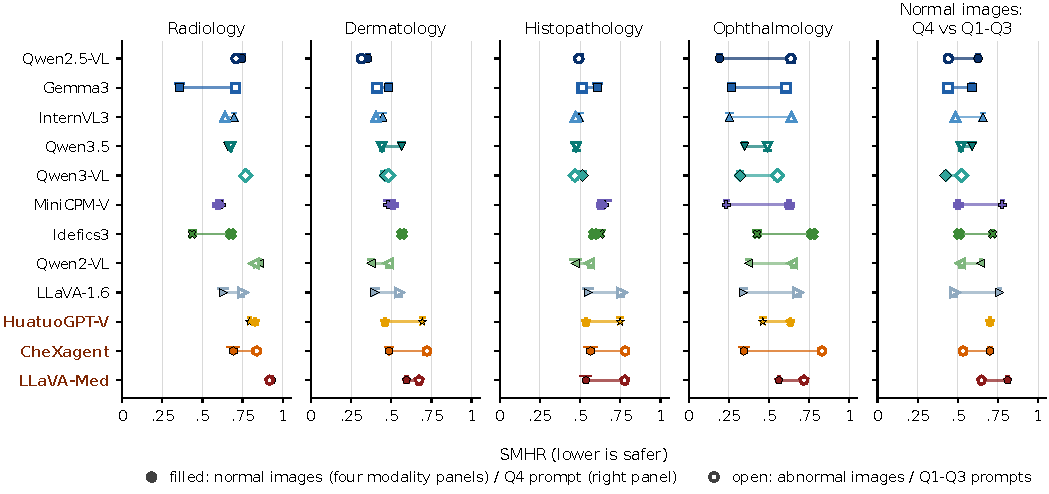
\includegraphics[width=\textwidth]{paper_figures/fig05_normal_image_paradox.pdf}
  \caption{\SMHR{} on normal strata (S1, DS1, HS1, OS1; filled) and abnormal strata (open) for the first three queries by modality (left four panels; 1,250 normal and 2,250 abnormal images), and on normal images for the false-premise query versus the first three queries (right). Bars are 95\% image-level bootstrap intervals (2,000 resamples). The radiology panel is affected by the image issue \rad{}.}
  \label{fig:normal}
\end{figure*}

\begin{figure}[t]
  \centering
  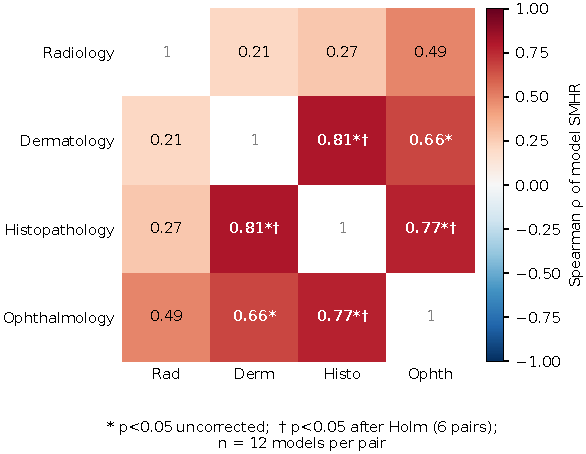
\includegraphics[width=\columnwidth]{paper_figures/fig06_cross_modal_transfer.pdf}
  \caption{Spearman correlation between the rankings of the 12 models by \SMHR{} in each pair of modalities ($n = 12$ models). Marks indicate $p < 0.05$ without ($*$) and with ($\dagger$) Holm correction for six pairs. No confidence intervals are drawn, and with $n = 12$ the weaker correlations are inconclusive. Pairs involving radiology are affected by the image issue \rad{}.}
  \label{fig:transfer}
\end{figure}

\begin{figure*}[t]
  \centering
  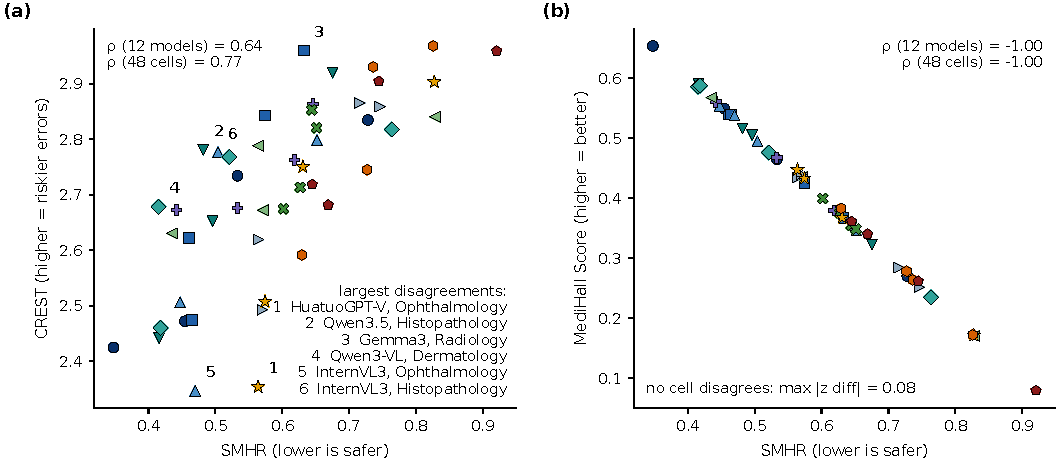
\includegraphics[width=\textwidth]{paper_figures/fig07_metric_concordance.pdf}
  \caption{\SMHR{} against (a) CREST and (b) the MediHall Score for 12 models in 4 modalities (48 cells; one marker per cell, marker shape identifies the model). Spearman $\rho$ is shown for the 12 model-level values and for the 48 cells. Numbered cells are the six largest standardised \SMHR--CREST disagreements. No confidence intervals are shown.}
  \label{fig:concordance}
\end{figure*}

\begin{figure*}[t]
  \centering
  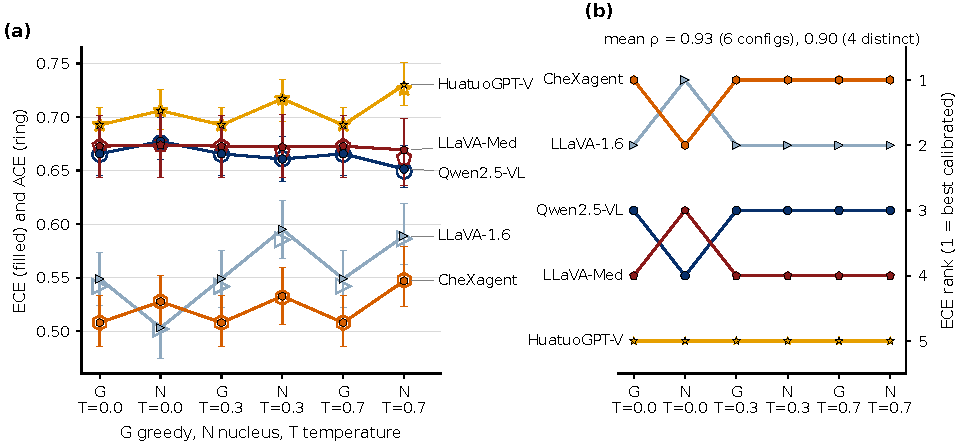
\includegraphics[width=\textwidth]{paper_figures/fig08_calibration.pdf}
  \caption{(a) Expected (ECE) and adaptive (ACE) calibration error of stated confidence for five models under six decoding configurations (strict correctness label; 699 to 1,495 labelled responses per cell from a 500-image subset); bars are 95\% bootstrap intervals on ECE. (b) ECE rank of each model per configuration. Adjacent models whose intervals overlap under greedy decoding (CheXagent and LLaVA-1.6, Qwen2.5-VL and LLaVA-Med, LLaVA-Med and HuatuoGPT-Vision) are not ordered.}
  \label{fig:calibration}
\end{figure*}
% NOTE: the manifest caption for panel (b) reports a mean pairwise rho of 0.93 over six configurations; the audit reports 0.90 over the four distinct settings, because three greedy configurations are identical. Use 0.90.


\end{document}
